\documentclass[12pt,letter]{article}
\usepackage[left=0.8in,right=0.8in,top=1in,bottom=1in]{geometry}
\usepackage{amsmath}
\usepackage{pdflscape}
\usepackage{amsfonts}
\usepackage{amssymb}
\usepackage{graphicx}
\usepackage{caption}
\usepackage{multicol}
\usepackage{multirow}
\usepackage{microtype}
\usepackage{euscript}
\usepackage{epsfig}
\usepackage{epstopdf}
\usepackage{mathrsfs}
\usepackage{tikz}
\usepackage{verbatim}
\usetikzlibrary{shapes,arrows}
\usetikzlibrary{positioning}
\tikzstyle{block} = [rectangle, draw, rounded corners]
\tikzstyle{line} = [draw, -latex']
\newcommand{\hypo}{\mathcal{H}}            
\bibliographystyle{ieeetr}

\usepackage[flushleft]{threeparttable}

%\usepackage[cp1251]{inputenc}
\usepackage[english]{babel} 
\DeclareMathOperator{\rank}{rank}
\newcommand*{\hm}[1]{#1\nobreak\discretionary{}
            {\hbox{$\mathsurround=0pt #1$}}{}}

            \def\onepc{$^{\ast\ast}$} \def\fivepc{$^{\ast}$}
\def\tenpc{$^{\dag}$}
\def\legend{\multicolumn{4}{l}{\footnotesize{Significance levels
:\hspace{1em} $\dag$ : 10\% \hspace{1em}
$\ast$ : 5\% \hspace{1em} $\ast\ast$ : 1\% \normalsize}}}


\newcommand{\bs}[1]{\boldsymbol{#1}}  
\newcommand{\bsA}{\boldsymbol{A}}

%\setstretch{1}                         
\flushbottom                            
\righthyphenmin=2                      
\pagestyle{plain}                       
%\settimeformat{hhmmsstime}  
\widowpenalty=300                   
\clubpenalty=3000                     
\setlength{\parindent}{0em}           
\setlength{\topsep}{0pt}              
\usepackage[pdftex,unicode,colorlinks=true,urlcolor=blue]{hyperref}
\usepackage{bbm}
\usepackage{tabularx}
\renewcommand{\emptyset}{\varnothing}

\setlength{\parskip}{0.5\baselineskip plus2pt minus2pt}

\newcommand{\e}{\varepsilon}
\DeclareMathOperator*{\Argmax}{\mathrm{Argmax}}
\DeclareMathOperator*{\Argmin}{\mathrm{Argmin}}
\DeclareMathOperator*{\argmax}{\mathrm{arg\,max}}
\DeclareMathOperator*{\argmin}{\mathrm{argmin}}

\newcommand{\blp}{\mathrm{BLP}}
\DeclareMathOperator*{\plim}{\mathrm{plim}}
\DeclareMathOperator{\Max}{\mathrm{Max}}
\newcommand{\R}{\mathbb{R}}
\newcommand{\Y}{\mathcal{Y}}
\newcommand{\Z}{\mathcal{Z}}
\renewcommand{\geqslant}{\geq}
\renewcommand{\leqslant}{\leq}
\newcommand{\p}{\bs p}
\newcommand{\y}{\bs y}
\def\dd#1#2{\frac{\partial#1}{\partial#2}}

\renewcommand{\emptyset}{\varnothing}


\DeclareMathOperator{\tr}{\mathrm{tr}}

\newcommand{\bb}{\bs \beta}
\newcommand{\X}{\bs X}
\DeclareMathOperator{\E}{\mathbb{E}}
\DeclareMathOperator{\PP}{\mathbb{P}}
\DeclareMathOperator{\V}{\mathbb{V}}
\DeclareMathOperator{\CM}{\mathbb{C}}
\renewcommand{\C}{\CM}
\DeclareMathOperator{\var}{\mathrm{var}}
\DeclareMathOperator{\cov}{\mathrm{cov}}
\DeclareMathOperator{\corr}{\mathrm{corr}}
\DeclareMathOperator{\MSE}{\mathrm{MSE}}
\DeclareMathOperator{\Bias}{\mathrm{Bias}}
\renewcommand{\P}{\PP}
\newcommand{\dsim}{\stackrel{d}{\sim}}
\newcommand{\hn}{\mathcal{H}_0}
\newcommand{\ha}{\mathcal{H}_a}
\newcommand{\thetab}{\bs \theta}
\newcommand{\pv}{\text{P-value}}
\newcommand{\N}{\mathcal{N}}
\newcommand{\MLE}{\scriptscriptstyle MLE}
\newcommand{\LR}{\mathrm{LR}}
\newcommand{\I}{\mathbb{I}}
\newcommand{\sumin}{\sum\limits_{i=1}^n}
\newcommand{\sumti}{\sum\limits_{t=0}^\infty}
\newcommand{\hbeta}{\hat{\beta}}
\newcommand{\halpha}{\hat{\alpha}}
\newcommand{\hsigma}{\hat{\sigma}}
\newcommand{\hvar}{\widehat{\var}}
\newcommand{\hcov}{\widehat{\cov}}
\newcommand{\Q}{\mathbb{Q}}



\newcommand{\pconv}{\xrightarrow{ \ p \ }}
\newcommand{\dconv}{\xrightarrow{ \ d \ }}
\newcommand{\asconv}{\xrightarrow{ \ a.s. \ }}
\newcommand{\msconv}{\xrightarrow{ \ m.s. \ }}

\newcommand{\pic}[4][h!]{\begin{figure}[#1]


\begin{center}\includegraphics[width=#2cm]{#3}\caption{#4\label{#3}}\end{center}
\end{figure}}

%outtex
\def\onepc{$^{\ast\ast}$} \def\fivepc{$^{\ast}$}
\def\tenpc{$^{\dag}$}
\def\legend{\multicolumn{4}{l}{\footnotesize{Significance levels
:\hspace{1em} $\dag$ : 10\% \hspace{1em}
$\ast$ : 5\% \hspace{1em} $\ast\ast$ : 1\% \normalsize}}}
%end outtex

%\bibliographystyle{ieeetr}

\newcommand{\laseq}{\stackrel{\lambda\text{-a.e.}}{=}}
\renewcommand{\d}{\underline}
\renewcommand{\u}{\overline}
\newcommand{\td}{\underline{\theta}}
\newcommand{\tu}{\overline{\theta}}
%\renewcommand{\theenumi}{\alph{enumi}}
%\renewcommand{\labelenumi}{(\theenumi)}
%\renewcommand{\theenumii}{\roman{enumii}}
%\renewcommand{\labelenumii}{\theenumii.}
%\renewcommand{\theenumiii}{\arabic{enumiii}}
%\renewcommand{\labelenumiii}{\theenumiii.}
%\renewcommand{\epsilon}{\varepsilon} 
\newcommand{\hneq}{\stackrel{\hn}{=}}
\newcommand{\deq}{\stackrel{d}{=}}
\title{Economics of Shotgun Marriage}
\author{Egor Kozlov\thanks{Economics Department, Northwestern University, egorkozlov2020@u.northwestern.edu. I thank my advisors Matthias Doepke, Martí Mestieri and David Berger for outstanding guidance and proofreading as part of my dissertation committee at Northwestern. I am grateful to Alessandra Voena for fantastic amount of help and support. I thank my colleagues Jane Olmstead-Rumsey, Kristina Manysheva, Bence Bardoczy, Stephanie Johnson and Gabriela Cugat, as well as all the participants of Macro Lunch at Northwestern for lots of helpful comments.}\\
{\small Northwestern University}}
\begin{document}
%\begin{center}\textbf{Economics 416-1} \\ \emph{By Egor Kozlov}\end{center}
\maketitle

\begin{abstract}
Many couples marry shortly after woman gets pregnant, that is often referred as a shotgun marriage. I show that in American Community Survey data couples who experienced a shotgun marriage, i.e. had their first child before or at the year of their marriage, divorce more often in the future.
%This feature is robust in different subpopulations, being relatively more pronounced for wealthier people, although the share of such marriages is lower among them.
I argue that this difference in divorce rates can be explained by endogenous selection into marriage: women who experienced unplanned pregnancy agree to enter marriages of lower quality. 
This implies that in the data having kids before marriage is a plausible proxy for having lower-quality marriage.
Then I show that these patterns in selection can be rationalized by the structure of childcare costs, where kids require both money and time, and disproportional exposure of women to these costs.
I estimate a structural model endogenizing marriage selection and use it to argue that causal impact of unplanned fertility shock,
%differences in marriage quality,
as opposed to different composition of the groups, drives the major part of the observable difference in divorce chances.
Qualitatively, this suggests that the main reason for poor performance of shotgun marriages is large, unexpected and heterogeneous childcare costs. Quantitatively, the model suggests sizable effects of risks of unplanned pregnancy on observable divorce rates, especially for young women.
\end{abstract}

\newpage

%[Paragraph 1: is shotgun marriage still a thing? Abstract - 2]
Term ``shotgun marriage'' is traditionally used to describe situations when having a baby triggers marriage of a couple. This practice does not solely refer back to more conservative times: in the modern US data around one-quarter of married women of age 21--40 had their first birth before or at the year of their first marriage. And, although it seems that abortion and contraception access would provide people with more choice, in this paper I show that in the data such couples still look like something pushed them to marry each other. In particular, their marriages appear less stable over time: despite of being less than quarter of the population shotgun marriage couples account for more than one-third of divorces. This paper has two main goals. First, I document and quantify the persistent difference in divorce rates of couples who experienced shotgun marriages and how it is pronounced for different population groups. Second, based on these findings I estimate a structural model that is capable of identifying importance of different channels that drive this difference.
%In this paper I argue that this pattern is rationalized by partners agreeing to enter marriages of lower quality as a response to unplanned pregnancy shock.

%[Paragraph 2: general importance? Child development]
Understanding the sources of variation in divorce rates is not just a household behavior question. For example, the divorces have large major impact on how people raise their children. The families who experienced shotgun marriages are often overlooked by the current literature focusing on child development. Growing up with a single mother or in a blended family (i.e. with step-parents) if conventionally considered\footnote{See Kearney, Levine 2017\nocite{kearney} for an extensive review of these issues} as a predictor of poor early and adult-life outcomes of the children, and those who have two married biological parents are typically not considered to be at risk. However, not all marriages are created equal, and treating all marriages equally may understate inequality: growing up in unstable marriage can be a predictor of ending up with a single mother or in a different household, as well as factor of risk by its own.

%[Paragraph 3: general importance? Other ideas]
In addition to child development impact of unstable marriages, divorces have other important consequences. For instance, they appear as an important driver of labor market choices and outcomes of women. Additionally, being divorced with young children is considered as lowering re-marriage prospective, and this can affect total fertility and marriage rates. Finally, the question of marriage selection and modeling divorces is curious by its own from prospectives of economic theory: if shotgun marriage predicts lower marriage quality and higher likelihood of divorce, we can use it as identifying variation for studying intra-household questions, that is relevant for developing realistic household models and understanding things that are not easy to observe directly.

%[Paragraph 4: general importance? We need to understand trends]
On more aggregate level, this paper can broaden the understanding of recent trends in household formation. First, around 40\% of new births in 2018 occurred by unmarried mothers. Second, increase in non-marital cohabitation is a documented trend, yet the median duration of cohabitation is 22 months\footnote{Source: Copen at al,  \cite{copen}}. Despite of this, unmarried unions with children are pretty rare: according to Payne, 2013\nocite{payne}, only about 3\% of children live in unions with unmarried cohabitating parents, as opposed to 21\% living with single mothers. Even mechanically this should suggest that large chunk of unmarried women transition into marriage shortly after they give births. Finally, this research can contribute to understanding differential behavior of marriage rates among racial and income groups, as the model identifies parameters of preferences and potential partners distribution, although it does not explicitly consider cohabitation that seems to become a substitute for married unions.

%[Paragraph 5: empirics --- what data do I use]
I use American Community Survey as the main dataset, as it has large sample sizes, uniform coverage and reports wide range of household and individual characteristics. One important drawback of it is that the marriage history in ACS is not reported perfectly, as it only has records of the year of the most recent marriage. I overcome this by conditioning on women who was married exactly once. I then use separate dataset of Survey of Income and Program Participation to re-establish the key findings without this restriction and show that this attrition does not introduce any important distortions besides changing magnitudes of what I refer to as divorce rates. Although SIPP provides superior coverage of the issues I study, the current work still mainly uses ACS: SIPP sample sizes do not allow to condition on multiple dimensions like child's age. 

%[Paragraph 6: empirics --- methodological issues shortly]
My main empirical contribution is describing association between having shotgun marriages and having a divorce, that I have not found to be explicitly discussed in the existing literature. Methodologically, the crucial comparison involves partitioning population of women who were married and had kids on two groups:  those who gave their first birth at least at the next year of their marriage (``marriage first'') and those who gave their first birth before or at the year of their marriage (``kids first''). I refer to the latter group as those who experienced a shotgun marriage. I additionally exclude from the comparisons women who had their birth more than five years before marriage, as they are increasingly likely to form a family with someone else than the child's father. 

%[Paragraph 7: empirica, findings --- main results]
The most important empirical result I show is substantially larger share of divorced people in ``kids first'' group. Although this difference is far from being causal, it is strong, robust to many ways of controlling for composition and is present among all subpopulations. Namely, chances of being divorced at the moment of survey are around twice larger for those who experienced a shotgun marriage as opposed to for those who did not ($18\%$ against $10\%$). This ratio reaches three for those who have college degrees, and is only around 1.25 for those who only finished a high school. When controlled for many confounding factors that include age, income, education and geography, as well as marriage duration and child's age, the difference in shares vanishes around a half, but remains large and statistically significant.  %Similar heterogeneity holds if I use woman's income instead of education, although defining and measuring income can be subtle in case of women with young children.

%[Paragraph 8: empirical findings --- duration, step-children, lf and child development outcomes]
Investigating the data further leads to few additional insights. First, different timing of marriage and marriage duration at the moment of survey between the two groups does not seem to be an important contributor to the difference. Second, the ``extra'' divorces we observe are concentrated around the time the child starts going to school. Third, for the cases when one can recover whether the child is step or own (it is not perfectly transparent in ACS samples), this status does not affect the marriage duration, moreover, less than fifteen percent of the couples I for which this is observed seem to have step-children as I exclude those women who had their births long ago after their marriage. [SIPP has better data to confirm these findings?]

%[Paragraph 7: model --- setup and why do we need a model]
These comparisons, however, contain lots of selection issues and unobservable heterogeneity, and to deal with it I set up a structural model that is capable of understanding of anatomy of the result. The model is based on growing branch of literature in dynamic household bargaining, and endogenizes savings, marriage and divorce decisions, fertility decisions and fertility shocks, together with the structure of childcare costs. The last element is crucial in generating heterogeneous response in terms of income or education: as time of wealthier parents is more expensive, unexpected childcare costs create relatively more distress for them. The model is estimated to match the key patterns of the data coming from American Community Survey, as well as supplementary sources, including ATUS and CEX for disciplining childcare costs part, and the structure I use fits the data well.

%[Paragraph 8: model --- what generates the result in theory]
The main driving force in the model is an unplanned pregnancy shock. Each period single people meet potential partners with some probability, and if the partner is met, couple decides whether to marry each other based on a simple bargaining procedure. The potential matches are heterogeneous in partner's characteristics and marriage quality, the latter is modeled as idiosyncratic joint utility gain of couple from being together, that can be interpreted as a ``love shock''.  Before the bargaining decision takes place, partners may or may not get an unplanned pregnancy shock, that proxies for unplanned children appearing in cohabitating unions as I do not model cohabitation explicitly. The shock interfers with bargaining: if the couple made a baby, woman risks to stay a single mother if the couple does not agree to marry. The conjecture is that in matches that experienced the shock women agree to enter the marriages of lower quality. Importance and even presence of this channel, however, depend on parameters of individual preferences and childcare costs that I estimate structurally.

%[Paragraph 9: model --- what I get from it, mechanics and anatomy]
The key conclusion of the estimation part is that couples who experienced an unplanned pregnancy shock indeed agree to enter the marriages of the lower quality, and this is the major driver of the number that we observe in the data. The model is capable of delivering various decompositions that split observable cross-sectional difference in divorce rates onto effects of age, marriage length, income, wealth and marriage quality. As it turns out, the last factor is the most important contributor to the difference, and its contribution is [of the similar magnitude than the observable difference]. Decomposing the result further, the model predicts that the major part of the difference in divorce rates is driven by couples who would not have married if they did not have a baby (i.e. who complied with the shock), although there is some additional distress of having an unplanned baby on those who would have married anyway.

%[Paragraph 10: model --- counterfactuals and speculative things]
Additionally, the estimated model delivers few nontrivial counterfactual predictions exploiting interaction between unplanned pregnancies and marriage quality. First, major part of divorces that happen early in life are seen as driven by unexpected pregnancies, though divorces happening later are not. Second, general impact of pressure of becoming a single mother on marriage decisions is substantial, and eliminating unexpected pregnancies happening before the marriage decision takes place lowers amount of people married by 25 by [...]. [Last, the model predicts decline in probabilities of unexpected pregnancies since 1980: the model matching fertility / marriage / divorce profiles from Census of 1980 predicts larger chances of unplanned pregnancies among all income and age groups.]

%[Paragraph 11: what I learned qualitatively]
As a general conclusion, the model teaches that conditional on enough observables, having kids before or at the year of marriage is a fairly good proxy for an inferior marriage quality, and therefore the difference in divorces between two groups is not purely explained by demography and economic outcomes. Therefore, observing similar people with slight difference in fertility timing may be informative about the questions of how marital stability affects people's economic choices and future outcomes of them and their children. Although this suggestion is model-based, many features of the actual data are consistent with it. This does not completely rule out preference and social arguments about different attitudes to divorce and childbearing, but suggests that large part of what we see can have solid economic reasoning, and, in particular, can respond to economic policy. 

%[Paragraph 12: what I learned about channels]
The main causal insight is that being single mother is a major threat affecting how people make their marriage decisions, and large and unequally distributed costs of raising young children can be a driver in creation of poor quality marriages. This channel can be of major importance for studying welfare policies subsidizing childcare, young families and single mothers, as well as for enforcing alimony payments and child support in general. This also emphasizes the link between contraception and abortion access and marriages, although this impact is limited as even the wealthiest couples do experience sizable share of shotgun marriages, though this may be cultural rather than economic issue.

%[Paragraph 13: not a paragraph, just table of contents]
I elaborate on these points in the following order. Section 1 of this paper discuss existing results and general trends that are already described by the literature. Section 2 discuss how I construct the dataset and timing variables, and Section 3 establishes main observations about differences in groups depending on their marriage timing, together with a number of additional considerations useful to understand the content of these differences. After that I explain theoretical model in Section 4 and the process of setting its parameters in Section 5. Section 6 describes estimation results and counterfactual simulations implied by these results. Section 7 provides more general discussion and concludes.

\section{Related Literature}

My work builds on few branches of literature, following long tradition of modeling fertility and marriage markets in family economics. I am not aware of any studies that cover precisely the narrow issue I focus on, but there are few recently established result that cover related aspects and compliment what I do. Three main building blocks that I utilize are literature on marriage selection and dynamic bargaining, few detailed lifecycle models of fertility and unplanned pregnancies and number of descriptive studies of microdata describing reduced form effects of out-of-wedlock births, trends in divorce rates and heterogeneity in time use of parents.

The main conceptual framework that I utilize are models of household's dynamic bargaining and limited commitment, extensively reviewed by Chiaporri, Mazzocco 2015.\nocite{chiappori-review} These models were used to answer various marriage and divorce related questions. Theoretical part of my model is mostly based on Voena, 2015\nocite{voena-1}, that uses dynamic bargaining to consider impact of changes in divorce laws, and Low et al, 2018\nocite{low-1}, focusing on marriage and divorce selection related to welfare utilitzation. There are few more recent papers utilitizing similar approaches, for instance, Shephard, 2019\nocite{shephard} studying gender and age pay gaps through equilibrium on marriage markets. 

To model fertility choices and shocks, I rely on recent lifecycle models. I make many choices similar to Sommer, 2015\nocite{sommer} who studies how changes in reproductive horizon affect couple's fertility decisions with in the environment with income shocks, paying detailed attention to time and money structure of childcare. More detailed treatment of unintended pregnancies is done by Ejrnæs, Jørgensen, 2018\nocite{ejrnaes}, they extend the model to allow for non-random abortion decisions though do not model childcare costs in details. 

Commitment in marriage and its interaction with fertility decisions attract recent attention as possible drivers of trends in marriage and divorce. Work by Lafortune, Low 2018\nocite{lafortune-1} uses ACS data and housing prices, as well as marriage market model, to argue that married people buy houses as a device to commit not to divorce, that allows them to secure investment in their future children. This is parallel and complimentary with my results, that mainly focus on consequences of not having enough commitment and how they relate to fertility timing. 

Impact of non-marital childbearing and parents divorce are well-documented empirically from children prospective. For example, Kearney, Levine 2017 use PSID to document how being born out of marriage statistically child's outcome in school years and in early adult life, and the heterogeneity of this by parent's education and age groups. Shortly, they find presence of ``marriage premium'' for children at each education level, though for less educated and younger mothers benefits of having married parents are more pronounced in early life, and for elder and more educated mothers --- in adult life. A classic study by Akerlof, 1996\nocite{akerlof} highlight the mechanism why unplanned pregnancies may not be aborted in couples so they are still present even with large abortion access. Finally, Ginther, Pollak, 2004 show that outcomes of children in blended families (i.e. having step-parents) are similar to outcomes of children of single parents. 

This paper fills an important gap in the literature considering impact of out-of-marriage births for women. As fertility, marriage and divorce involve many individual decisions affected by many unobservable factors, it is not possible to ask casual questions by using only the data, and existing empirical studies only provide descriptive evidence. This study contributes to the growing literature of quantitative models that both use the tools of family economics to endogenize timing of fertility, marriage, divorce and their interactions, and, on the other hand, provide numbers and patterns consistent with microdata, so they can be used to answer policy questions.

As noted by Ginther and Pollak, causal questions in the context of marriage and divorce should be taken with caution: to answer, for instance, how parents' divorce affect child's future we have to be precise what counterfactual we compare it with (either parents never divorced, parents stayed together for few more years, parents never married). The same issues concern impact of unplanned pregnancies in cohabitating couples, therefore, instead of trying to ask causal quesitons I the main goal of using the model is to deliver counterfactual outcomes, that still facilitate understanding of some causality.

\section{Empirical Facts}

This section presents key empirical facts and several exercises on testing their validity. In summary:
\begin{enumerate}
\item Women who had their first child before their first marriage (K$\to$M) are more likely to be divorced than those who had their first child in their first marriage (M$\to$K).
\item Relative difference in the share of divorced between K$\to$M and M$\to$K is increasing with income and education
\item These results are statistically significant and robust to various methods of controlling for observable composition of the groups
\end{enumerate}

To establish these results, I mainly use American Community Survey (ACS), that has large sample sizes and many relevant observable characteristics of households. Its only limitation is that it does not recover marriage and fertility history perfectly. Because of this, I re-confirm the results with the data from Survey of Income and Program Participation (SIPP 2014), that has fewer observations but more detailed marriage and fertility history.

I begin with describing empirical strategy, then Section \ref{keycomp} presents the key results for ACS and SIPP, the following sections present several validity checks.

\subsection{Defining Groups}

General strategy involves dividing sample in two groups: couples who had kids before their marriage ($K\to M$) and those who had kids after their marriage ($M\to K$). After this division I perform multiple comparisons of these groups: the main comparison is looking at divorce rates in several variations, few additional comparisons involve marriage inequality and outcomes of children.

Although the couples are the primary focus of the paper, the surveys I use look at individuals and households. Therefore I follow females rather than males: upon divorce, children are more likely to stay with mothers (share of single mothers in ACS is ..., single fathers ...). The timing I consider in the  most general form is (for females, given both events occurred): 
\[\Delta T = T^{\text{First child  is born}} - T^{\text{First marriage happened}},\]
where $T$ refers to moments of time. After that I define two groups (given $\Delta T$ is measured in years):
\begin{align*}&M\to K \Leftrightarrow \Delta T \in \{1,2,...\},\\
&K\to M \Leftrightarrow \Delta T \in \{...,-2,-1,0\},\end{align*}

In practice, I exclude observations with $\Delta T < -5$ or $\Delta T > 10$. The reason for the first one is mainly related to step-children: for the subsample when it can be tracked, share of step-children is becomes higher with more negative $\Delta  T$ in ACS, and having step-children that are relatively adult at the moment of marriage is a complex issue that is beyond the scope of the paper. See a note ... in the appendix about this. The reason for the second one is mainly data quality (...).

As the evidence is mainly cross-sectional, I refer to share of divorced people in a group as divorce rates. Unlike fertility, people can change their marriage status all the time, so there is no such thing as completed divorce rate, therefore I just use the share of people who ever had a divorce. More accurate measuring of divorce rates involves conditioning on age, however fixing age restricts the attention to a particular cohort, and pooling people of different ages together allows to think about more general population.


\subsection{Sample Restrictions}
\subsubsection{ACS data}
I take ACS samples of 2008--2016, as only they have variables concerning the duration of current marital status. Namely, people report the year of their most recent marriage. Fertility history is not observed perfectly: the survey reports age of the eldest child residing with individual. However, both of these variables can recover the timing of interest for relatively large subpopulation of females who:
\begin{enumerate}
\item Had exactly one marriage, so they are either married or divorced now (treating legally separated, spouse absent and widowed as married)
\item Have children present in household, with age of the eldest child below 18
\item Most likely reside with their eldest child judging by mother's age (I pick 21--40)
\end{enumerate}
%The last restriction can be relaxed, but it allows to track partners and children more clearly and also insures better quality of self-reported data.

The most important restriction here is being married once --- that means that people who re-marry drop out of sample. For instance, if it take longer to re-marry for the people who had kids before their first marriage, share of divorced people in the group $K\to M$ would be larger without differences in probability of their first marriage to dissolve. This concern can only partially be addressed with ACS data, but this is not an issue in SIPP. 


All mean and quantile calculations are performed using person weights.

\subsubsection{SIPP data}

I use wave 1 of 2014 SIPP. It it representative for the whole population, I use person weights in all calculations.

SIPP has much more detailed information on marital history and fertility: it explicitly asks about times of first marriage and first births, it also asks about multi-partner fertility. However it has substantially smaller sample size. For SIPP I relax the restrictions and consider all females who had at least one marriage and are of age 20--40 (treating married with spouses absent, separated and widowed as married), as their marital and fertility history is recovered perfectly.

%When dividing people by income, however, I have to further restrict attention to households that consist of mother + spouse/partner (if reported) + children. This creates some attrition especially for young people, but differences in defining household members are minimal between ACS and SIPP, so it is not likely that it creates an issue.

\subsection{Income Partition\label{inc-part}}
I define income groups based on per hour income of working females, by excluding those who does not work or work too little from income considerations. Precisely, I define working as those who are employed now, report to work more than 25 weeks in the last year, report non-missing labor income above or equal to $\$1000$ per year, report non-missing usual working hours above or equal to $5$ hours per week.

As weeks worked last year are defined only on intervals for ACS, I impute them using the midpoints of respective intervals, then define yearly hours as a product of usual hours and imputed weeks worked. This allows to define log per-hour income as log-difference of yearly log wage and salary income with yearly log hours. I residualize these income data by regressing it on 4th degree polynomial in age, dummies and linear trends in age for each US state and dummies for each ACS survey year.

In SIPP 2014, I perform the similar operations. I exclude females who had less than $1000/12$ monthly income or had average weekly hours less than 5 during the last month. Then I divide monthly income on four times average weekly hours to get estimate for per-hour earnings. As before, I residualize logs of these income by regressing them on the same factors, except that instead of year controls (I only use 2014) I use month controls.

\subsection{Raw Comparisons\label{keycomp}}
The main results I discuss is summarized by Figure \ref{shrs} for ACS and Figure \ref{shrs-sipp} for SIPP. Table \ref{diff-raw} in presents these results in numbers.


\begin{figure}[h!]
\centering
\includegraphics[width=0.8\linewidth]{shrs.eps}
\begin{tabular}{|p{0.65\linewidth}|}
\hline
\footnotesize $\Delta T = \text{Year}^{\text{first child}} - \text{Year}^{\text{first marriage}}$. Restriction: $\Delta T \in \{-5,...,10\}$\\
\footnotesize Definition: K$\to$M if $\Delta T \in \{-5,...,0\}$. M$\to$K if $\Delta T \in \{1,...,10\}$.\\\hline
\end{tabular}
\caption{Share of K$\to$M couples and share of divorced, ACS\label{shrs}}
\end{figure}



\begin{figure}[h!]
\centering
\includegraphics[width=0.8\linewidth]{shrs-sipp.eps}
\caption{Share of K$\to$M couples and share of ever divorced, SIPP\label{shrs-sipp}}
\end{figure}


\begin{table}[p]
\begin{center}
\begin{tabular}{l c  c c  c  c c}\cline{2-7}
\multicolumn{1}{c }{} & \multicolumn{3}{c  }{\small ACS: sample of married once} & \multicolumn{3}{c }{\small SIPP: sample of ever married} \\\cline{2-7}
\multicolumn{1}{c }{}  & \small{\textbf{share of}} & \multicolumn{2}{c  }{\textbf{divorced (now)}} & \small{\textbf{share of}} & \multicolumn{2}{c }{\textbf{divorced (ever)}} \\\cline{3-4}\cline{6-7}
\multicolumn{1}{c }{}  & \small{\textbf{kids-first}}  &\small marriage-first &  \small kids-first & \small{\textbf{kids-first}} & \small marriage-first & \small kids-first \\\hline\hline
\textit{All females, 21--40}  & $23.2$ & $10.1$ & $18.0$ & $22.8$ & $24.1$ & $34.8$ \\
\textit{All females, 35--40} & $18.0$ & $11.3$ & $23.0$ & $18.9$ & $28.1$ & $45.5$ \\\hline\hline
\multicolumn{7}{p{0.9\linewidth}}{ \textbf{Education partition}}\\\hline
\textit{High school only, 21--40} & $34.2$ & $13.9$ & $17.2$ & $33.4$ & $29.2$  & $34.2$ \\
\textit{College graduates, 21--40} & $\phantom{0}9.9$ & $\phantom{0}5.3$ & $14.7$ & $10.5$ & $12.9$ & $27.5$ \\\hline\hline
\multicolumn{7}{p{0.9\linewidth}}{ \textbf{Income partition:} subsample of working women}\\\hline
\textit{Low 30\% income, 21--40} & $30.8$ & $17.6$ & $24.1$ & $34.6$ & $30.5$ &  $42.5$ \\
\textit{Mid 40\% income, 21--40} & $25.5$ & $14.2$ & $21.5$ & $24.1$ & $28.3$ & $45.8$ \\
\textit{Top 30\% income, 21--40} & $14.1$ & $\phantom{0}7.7$ & $18.1$ & $12.4$ & $22.9$  & $32.8$ \\\hline\hline
\multicolumn{7}{p{\linewidth}}{ \footnotesize \textit{Notes:} Kids-first refers to women whose year of marriage is 0 to 5 years after their year of the first birth. Marriage-first refers to women whose year of marriage is 1 to 10 years after their year of the first birth. Women outside of these two groups are excluded. Income here refers to residualized per-hour income for subsample of working women, as described in Section \ref{inc-part}. ACS is American Community Survey, 2008--2016. SIPP is Survey of Income and Program Participation, 2014.}\\\hline
\end{tabular}
\caption{Percentages of kids-first group and percentages of divorced in each group by subpopulations. ACS and SIPP (repeats Figures \ref{shrs} and \ref{shrs-sipp}) \label{diff-raw}}
\end{center}
\end{table}

Three key observations from the table are:
\begin{enumerate}
\item About one-fifth of females have their first kid before or at the year they marry, this share quickly decreases with income and education
\item Share of divorced people among those who had their first kid before on at the year of their first marriage is larger.
\item The share of divorced people is about 1.5 higher for low income/education females and more than twice higher for high income/education.
\item The ACS result is not likely to be driven by picking only people with one marriage, as the pattern is exactly the same if I use SIPP and count for remarriages
\end{enumerate}

This alone is not enough to draw strong conclusions: composition of these groups is drastically different. For instance, as suggested by the table, people with lower income are more likely to get divorced, so even conditional on income/education group K$\to$M couples may be poorer with each subgroup. Additionally, many other factors may drive the differences, including different ages of children (people in K$\to$M group by construction have older babies after any given number of years after marriage), regional and racial differences in attitudes to divorce, age composition, possible presence of step-children in K$\to$M couples and so on. I attempt to control for few of these things and argue that they explain these differences only partially, that suggests the presence of causal mechanism that I describe.

\subsection{Adjusting for Composition\label{adcomp}}
As people in K$\to$M and M$\to$K groups obviously have different characteristics, as in particular suggested by Figure \ref{keycomp}, I use regression techniques to see what part of difference is attributed to this composition. Appendix \ref{comp-diff-appendix} quantifies these differences, shortly, people in K$\to$M group are younger, less educated, have kids earlier, marry slightly earlier and have more unequal marriages. In this part I control for difference in observable characteristics to see what part of the difference is attributed to the fact of being in K$\to$M group. Shortly, controlling for observables mitigate some part of the difference but it still remains sizable and significant.

In general, I perform the following exercise: I regress indicator of female being divorced on set of controls $X$ and dummy variable $\I(\text{K$\to$M})_i$. The specification I use is
\[D_i = \Delta \cdot \I(\text{K$\to$M})_i + X_i\gamma + \varepsilon_i.\]
Replacing $X_i$ with a constant corresponds to raw mean comparison described above. 

I report three possible estimates of $\Delta$:
\begin{itemize}
\item \textbf{Raw}, corresponding to differences in raw means in the previous part
\item \textbf{Controls}, where the regression includes dummies for ACS year, the US state, number of children, number of years after marriage, age of the eldest child, race and education group + 4th degree polynomial in woman's age
\item \textbf{Controls+income}, where the regression includes all of the above + 3rd degree polynomial in log female per-hour income (residualized as described above) for subsample of working women. This subsample is smaller, but has arguably better data quality.
\end{itemize}

See Table \ref{diff-contr} for the results. Generally, controlling for composition decreases observable difference, but this decrease is less than half in magnitude: even controlling for many observable factors, many of which may itself be results of unplanned fertility, we cannot assign all observable difference to composition of the groups. This also implicitly suggests that the income partition I choose makes sense: conditional on income group, additional controlling for income does not change the observable coefficient much. 

\begin{table}
\begin{center}
\begin{tabular}{l c  c c c c c c}\cline{2-8}
\multicolumn{1}{c}{} & \multicolumn{7}{c}{ACS: sample of married once}\\\cline{2-8}
\multicolumn{1}{c}{} & \small Share of &\multicolumn{2}{c}{\small raw difference} & \multicolumn{2}{c}{\small with controls \,\,\, \,\,\,} & \multicolumn{2}{c}{\small controls + income} \\ \cline{3-8}
\multicolumn{1}{c}{} & \small divorced & $\Delta$ & (s.e.) & $\Delta$ & (s.e.) & $\Delta$ & (s.e.) \\\hline\hline
\textit{All females, 20--50} & 14.3 &  \phantom{0}7.9 &   (0.1) &    5.7  &    (0.2) &     4.6   &   0.2 \\
\textit{All females, 35--40} &  17.3 &  11.7  &  (0.2) &   6.7 &  (0.3) &     6.2  &   (0.4) \\\hline\hline
\multicolumn{8}{p{0.6\linewidth}}{\textbf{Education partition}}\\\hline
\textit{High school only, 20--50} & 18.1 &   \phantom{0}3.3  &    (0.2) &   8.4 &   (0.3)   &  7.8   &  (0.5) \\
\textit{College graduates, 20--50} & \phantom{0}8.5 &   \phantom{0}9.4 &   (0.2) &   3.9 &   (0.3) &   3.2   &  (0.4) \\\hline\hline
\multicolumn{8}{p{0.6\linewidth}}{\textbf{Income partition:} subsample of working women.}\\\hline
\textit{Low 30\% income, 20--40} &  21.6 &  \phantom{0}6.5 &    (0.3) &    7.8 &  (0.5) &   7.8   &  (0.5) \\
\textit{Mid 40\% income, 20--40} &  17.1 &  \phantom{0}7.3 &   (0.3) &    3.6   & (0.4) &   3.6 &    (0.4) \\
\textit{Top 30\% income, 20--40} & 11.1 &  10.4 &  (0.3) &    3.5 &   (0.4) & 3.5 &  (0.4) \\
\hline
\multicolumn{8}{p{0.9\linewidth}}{ \footnotesize \textit{Notes:} here $\Delta$ is defined as coefficient in cross-sectional regression
$\text{Divorced}_i = \Delta \cdot \text{Kids-First}_i + \gamma X_i + \varepsilon_i$,
where ``Raw difference'' refers to regression with no $X_i$ that corresponds to the difference in means in Table \ref{diff-raw}. Controls are described in Section \ref{adcomp}. Coefficients and standard errors are multiplied by 100 so they refer to percents.}\\\hline
\end{tabular}
\caption{Percentage difference in shares of divorced, raw and adjusted for composition via regression, ACS data.\label{diff-contr}}
\end{center}
\end{table}

\subsection{Additional Comparisons}

Appendix \ref{extra-comparisons} shows few additional graphs and exercise. I summarize their results here:
\begin{enumerate}
\item In the sample I use M$\to$K women are married for longer at the moment of survey\footnote{This does not contradict the fact that K$\to$M couples marry slightly earlier as I use the sample of married women.} (so they had \emph{more} years to break up), comparing marriages of the same duration only exacerbates the difference.
\item Children of K$\to$M women are on average older (as they are born in earlier ages). Divergence between K$\to$M and M$\to$K observable divorce probabilities happens around ages 5--10. After controlling for composition, however, I show that K$\to$M couples divorce more often even conditional on child's age.
\item To further address concerns about duration, I recompute the numbers using getting the divorce at the year of survey, corresponding to marginal divorce probability as opposed to cumulative divorce probability (being divorced at by the moment survey). The magnitudes and patterns are very similar, though the numbers are harder to interpret. This suggests that 
\item I show that the difference is not likely to be driven by presence of stepchildren in K$\to$M families. In fact, as I restrict $\Delta T \geq -5$, share of stepchildren is relatively small, and surviving couples with stepchildren do not differ in observable marriage duration with couples without stepchildren.
\end{enumerate}

\subsection{Intra-Household Allocations [TBD]}
I document few additional facts describing the difference between K$\to$M and M$\to$K besides being divorced. Following Lafortune et al, 2018, I construct measure of children's grade retention based on ACS (that is an indicator if any school-age child in the household is in grade that is lower than prescribed by her/his age). I show this together with few other intra-houeshold characteristics: measure of inequality and labor force participation. 

See Table \ref{intra} for the numbers. The exercise suggests that children on K$\to$M women repeat grades significantly more often, and this happens even in higher-income households. [This table is based on old sample so it is slightly inconsistent with what I do above, I will redo this in one of the future iterations.] 

\begin{table}
\centering
\begin{tabular}{l  c c  c c }
\cline{2-5}
& \multicolumn{2}{ c  }{\footnotesize \textit{All couples}}  & \multicolumn{2}{ c }{\footnotesize \textit{Top 40\% of income} } \\\hline
&                       \footnotesize  Marriage-first & \footnotesize Kids-first &  \footnotesize  Marriage-first & \footnotesize  Kids-first \\\hline
\footnotesize \textit{Female in Labor Force}        & $70.3$  & $71.4$  & $79.3$ & $85.3$  \\\hline
\footnotesize \textit{Earninigs Ratio}    &  $95.2$ & $93.9$  &  $95.8$ &  $96.4$ \\\hline
\footnotesize \textit{Kids' Grade Retention}  & $\phantom{0}4.6$    & $\phantom{0}7.6$ &   $\phantom{0}3.3$   & $\phantom{0}5.9$ \\\hline
\end{tabular}
\caption{Child's outcomes and intra-household allocations, all numbers are in percents.\label{intra}} %[This is borrowed from an old draft so its methodology is slightly inconsistent, to be fixed later]\label{intra}}
\end{table}

%\section{Mechanisms}
%This part describes the mechanism I am trying to capture in the model that is presented in the following section. Suppose single agents with characteristics $\omega^m$ and $\omega^f$ can meet each other and form a couple. On top of individual characteristics, let couples be characterized by idiosyncratic utility gain $\psi$ from being together, that can be interpreted as a love shock. Let also there exists a variable $\theta$ that describes terms of marriage (that can be interpreted as decision weight of wife in a collective household). Let for $i \in \{f,m\}$ functions $V^{i,c}$ and $V^{i,s}$ denote values of being in a couple and being single, respectively. People agree to marry if there exist marriage terms $\theta$ such that gains of both spouses from marriage is positive, that is
%\[\Delta^f = V^{f,c}(\omega^f,\omega^m,\theta,\psi) - V^{f,s}(\omega^f) \geq 0, \ \ \Delta^m = V^{m,c}(\omega^f,\omega^m,\theta,\psi) -  V^{m,s}(\omega^m) \geq 0.\]
%
%Assume that utilities of potential spouses increase in $\psi$. Assume also that wife benefits from higher $\theta$ and husband benefits from lower $\theta$. The following illustration captures the intuition for the model: 



\section{Model}

% This is part of draft.tex containig the model
% \section{Model}
The model is a mixture between conventional heterogeneous agents savings model (Bewley--Huggett--Aiyagari framework) and household formation and dynamic bargaining, that is extensively surveyed by Chiaporri, Mazzocco 2015. 

Agents live for $T$ periods. The agents are males, females and married couples. Couples can have a child together, and if a couple with a child divorces up, the child stays with mother, and this is how singe females can have kids. Single females with kids randomly re-enter marriage market by becoming single females without kids.\footnote{The reason for this assumption is to avoid modeling mixture between step and own children, and the fact that single mothers are not a main focus of the paper.}


Single people without kids randomly meet partners with characteristics similar to them and decide whether to create a couple. Couples agree on some marriage terms, represented by each spouse's weight in couple's objective function. The rationale for marriage includes risk-sharing, returns to scale in consumption, possibility to have a child in the future and additional utility surplus of being married (love shock). Each period after random shocks are realized, couples may decide to renegotiate their marriage terms if one of the spouses is better off being single. If they cannot find marriage terms that are satisfactory for both, divorce happens.

Couples can choose to have a child and can also experience unplanned pregnancies. Unplanned pregnancies cannot be aborted, but the arrival rate of unplanned pregnancies depend on woman's productivity as well as on age. In addition to couples, single people who met each other may experience an unplanned pregnancy just before they decide whether to create a couple. In this case, upon disagreement the female becomes a single mother. This mechanism is a stylized representation of kids appearing in unmarried cohabitating couples: since I do not model cohabitation, those kids appear just before people actually decide to marry each other.

Figure \ref{transitions} summarizes the discussed transitions.

\begin{figure}
\begin{center}
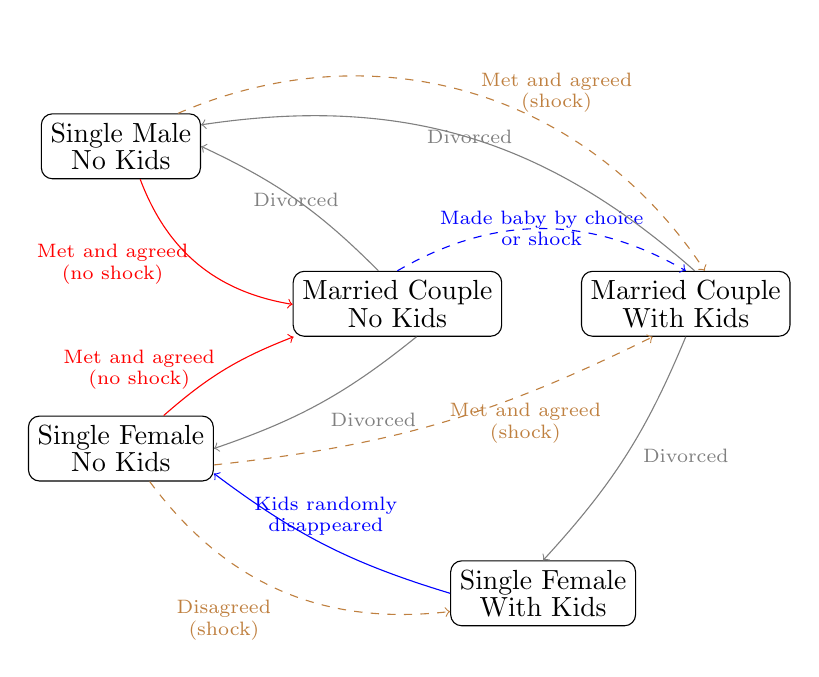
\begin{tikzpicture}[every text node part/.style={align=center}]
   % Place nodes
   \node [block] (1) {Single Female\\[-0.5ex]  No Kids};
   \node [block, above right = 1cm and 1cm of 1] (2) {Married Couple \\[-0.5ex] No Kids};
   \node [block, right = of 2] (3) {Married Couple \\[-0.5ex] With Kids};
   \node [block, above = 3cm of 1] (4) {Single Male  \\[-0.5ex]  No Kids};
   \node [block, below right = 1cm and 3 cm of 1]  (5) {Single Female\\[-0.5ex]  With Kids};
  
   \draw[->, color = red] (1) to [bend left = 10] node [left] {\scriptsize Met and agreed \\[-1ex] \scriptsize (no shock)} (2);
   \draw[->, color = brown, dashed] (1) to [bend right = 30] node [below left] {\scriptsize Disagreed \\[-1ex] \scriptsize (shock)} (5);
   %\draw[->, color = red] (1.210) to [bend right=90]  node [below] {\scriptsize Did't meet or \\[-1ex]  \scriptsize disagreed (no shock) } (1.330);
    \draw[->, color = brown, dashed] (1.350) to [bend right=10]  node [right] {\scriptsize Met and agreed \\[-1ex]  \scriptsize (shock) } (3.225);
    \draw[->, color = red] (4) to [bend right = 30] node [left] {\scriptsize Met and agreed \\[-1ex] \scriptsize (no shock)} (2);
     \draw[->, color = brown, dashed] (4.30) to [bend left = 40] node [right] {\scriptsize Met and agreed \\[-1ex] \scriptsize (shock)} (3.60);
    %\draw[->, color = red] (4.150) to [bend left=90]  node [above] {\scriptsize Did't meet or disagreed} (4.30);
    \draw[->, color = blue, dashed] (2.90) to [bend left=30] node  {\scriptsize Made baby by choice \\[-1ex] \scriptsize or shock} (3.90);
    \draw[->, color = gray] (2.120) to [bend right=10] node {\scriptsize Divorced} (4.0);
    % \draw[->, color = gray, dashed] (2.270) to [bend left=20] node [above right] {\scriptsize Divorced  \\[-1ex] \scriptsize + became pregnant } (5.90);
    \draw[->, color = gray] (2.300) to [bend left=10] node [below right] {\scriptsize Divorced} (1.0);
  \draw[->, color = gray] (3.75) to [bend right=25] node  {\scriptsize \ Divorced} (4.15);
  \draw[->, color = gray] (3.270) to [bend left=10] node [right] {\scriptsize \ Divorced} (5.90);
    \draw[->, color = blue] (5.180) to [bend left=10] node [above] {\scriptsize Kids randomly \\[-1ex] \scriptsize disappeared} (1.345);
\end{tikzpicture}
%\begin{tabular}{ p{\linewidth} }
%\footnotesize \emph{Note}: this captures key transitions between discrete states before individuals retire. \\
%\end{tabular}
\caption{ Summary of important transitions \label{transitions} }
\end{center}
\end{figure}


\subsection{Remarks on Notation}
I write $V^{i,j}$ to represent individual value functions in the model. Here $i$ represents gender: $f$ for female or $m$ for male. $j$ represents demographic status: $s$ for singles without kids, $sk$ for singles with kids (females only), $c$ for couples without kids and $ck$ for couples with kids. Couple's joint value functions have only one superscript $j \in \{c,ck\}$. Relation between joint value function $V^{c}$ and each spouse's value functions $V^{m,c}$ and $V^{f,c}$ is described in details in couple's section.

\subsection{Singles Without Kids}
Singles without kids are characterized by age $t$, labor productivity $z$ and assets (savings) $a$. I use $\omega = \{z,a\}$ to individual characteristics other than age.

Each period single individuals meet a partner of the same age and characteristics $\omega^p$ with probability $p^{\text{meet}}_t$. If meeting happens, with probability $p^{\text{preg}}_t$ unplanned pregnancy happens. After realizing new period's shocks and pregnancy status couple tries to negotiate marriage terms. If they found marriage terms that are satisfactory for both ($m^{np} = 1$ in case of no pregnancy or $m^p = 1$ in case of pregnancy), they form couple with characteristics $\Omega^c$ . If satisfactory marriage terms could not be found, the individual stays single, or becomes single mother if she is female and unplanned pregnancy happened.

The value function of male agent therefore is
\begin{align}V^{m,s}_t(\omega) = \max\limits_{c} & \bigg\{ u(c) + \beta \E_t \Big[ (1 - p^{\text{meet}}_t)\cdot V^{m,s}_{t+1}(\omega') + \\ \nonumber
& \hspace{7em} p^{\text{meet}}_t (1-p^{\text{preg}}_t) \big\{ m^{np} \cdot V^{m,c}_{t+1}(\Omega^c) + (1-m^{np})V^{m,s}_t(\omega')\big\} + \\  \nonumber
& \hspace{10em} p^{\text{meet}}_t p^{\text{preg}}_t \big\{ m^{p} \cdot V^{m,ck}_{t+1}(\Omega^c) + (1-m^{p})V^{m,s}_{t+1}(\omega')\big\}  \Big]  \bigg\},\\  \nonumber
 \end{align}\vspace{-3em}
 \begin{align*}
 \text{s.t. \ }  &  a' = R\cdot a  + W^m_t(z) - c  & \text{ (evolution of assets)}\\
 &  z' = z + \varepsilon^{z,m}_t, \ \ \varepsilon^{z,m}_t \sim \mathcal{N}(0;\sigma_{z,m}^2) &  \text{ (evolution of productivity)}\\
  & \log W^m_t = z_t + \text{Trend}^m_t, \ \ \  \text{Trend}^m_t = a^m_0 + a^m_1\cdot t  +  a^m_2 \cdot t^2 &  \text{ (labor income and trend)}\\
  & \Omega^c = \mathcal{M}^m(a',z') &  \text{ (marriage prospectives)}
\end{align*}
where random function $\mathcal{M}^m$, representing characteristics of potential couple is defined in Section [...].

The value function of female agent is
\begin{align}V^{f,s}_t(\omega) = \max\limits_{c} & \bigg\{ u(c) + \beta \E_t \Big[ (1 - p^{\text{meet}}_t)\cdot V^{f,s}_{t+1}(\omega') + \label{single-fem} \\  \nonumber
& \hspace{7em} p^{\text{meet}}_t (1-p^{\text{preg}}_t) \big\{ m^{np} \cdot V^{f,c}_{t+1}(\Omega^c) + (1-m^{np})V^{f,s}_t(\omega')\big\} + \\  \nonumber
& \hspace{10em} p^{\text{meet}}_t p^{\text{preg}}_t \big\{ m^{p} \cdot V^{f,ck}_{t+1}(\Omega^c) + (1-m^{p})V^{f,sk}_{t+1}(\omega')\big\}  \Big]  \bigg\},
\end{align}\vspace{-3em}
\begin{align*}
 \text{s.t. \ }  &  a' = R\cdot a  + W^f_t(z) - c  & \text{ (evolution of assets)}\\
 &  z' = z + \varepsilon^{z,f}_t, \ \ \varepsilon^{z,f}_t \sim \mathcal{N}(0;\sigma_{z,f}^2) &  \text{ (evolution of productivity)}\\
  & \log W^f_t = z_t + \text{Trend}^f_t, \ \ \  \text{Trend}^f_t = a^f_0 + a^f_1\cdot t  +  a^f_2 \cdot t^2 &  \text{ (labor income and trend)}\\
  & \Omega^c = \mathcal{M}^f(a',z') &  \text{ (marriage prospectives)}
\end{align*}

% 
The crucial difference here is the term $V^{f,sk}$: it reflects the fact that upon disagreement woman becomes a single female with a child. 

\subsection{Couples Without Kids}
Couple is characterized by age $t$ (assumed the same for both spouses), marriage terms $\theta$, productivities of female and male $z^f$, $z^m$ and additive marriage surplus $\psi$. Couple maximizes weighted expected lifetime utility, and $\theta$ represents share of female in this objective function, therefore $\Omega = \{\theta,\psi,z^f,z^m\}$ represent characteristics of couple.

The key element shaping couple's decisions is participation constraints: each period the expected lifetime utility of staying in couple should be not less that expected lifetime utility of getting a divorce and becoming a single agent. Depending on realization of the shocks, if it is possible to satisfy both participation constraints the next period (so no divorce happens, $d = 0$) state is $\Omega'$. If participation constraints cannot be satisfied, the couple gets a divorce $d = 1$ and its characteristics are dissolved onto $\omega^{df}$ and $\omega^{dm}$.  In more details this is described in Section [...].

Fertility dimension is an important element. Each period couples get fertility shock $p^{\text{preg}}_t$. If it happens, they become couple with a child if they stay together (renegotiation happens after they know realization of the shock), or become single male and single female with a child if they do not. If the shock does not happen, they still may make a decision to get a baby \emph{after} they renegotiate the marriage terms if they stay together. This timing is subtle, but is required for everything to be internally consistent, see Appendix ... for more details on how timing interacts with renegotiation. 

After realization of all the shocks and making fertility and divorce decisions in the current period the problem of the couple that stays childless is
\begin{align}& \hspace{5em}  V^{c}_t(\Omega) = \max\limits_{c^f,c^m}  \bigg\{ \theta\cdot u(c^f) + (1-\theta)\cdot u(c^m) + \psi +  \label{vf-c} \\   \nonumber
 &  \beta \E_t \Big[   (1 - p^{\text{preg}}_t)\cdot \left\{ (1-d^{\text{np}})\cdot \max\left\{ V^{ck}_{t+1}(\Omega'),V^{c}_{t+1}(\Omega')\right\} + d^{\text{np}}\cdot [ \theta V_{t+1}^{f,s}(\omega^{df}) + (1-\theta)V_{t+1}^{m,s}(\omega^{dm})]\right\}  +  \\  \nonumber
& \hspace{5em} p^{\text{preg}}_t\cdot \left\{ (1-d^{\text{p}})\cdot V^{ck}_{t+1}(\Omega') + d^{\text{p}}\cdot [ \theta V_{t+1}^{f,sk}(\omega^{df}) + (1-\theta)V_{t+1}^{m,s}(\omega^{dm})]\right\} \Big] \bigg\},
\end{align}\vspace{-2em}
\begin{align*}
\text{s.t. \ }& a' + c = R\cdot a  + W^m_t(z^m) + W^f_t(z^f) & \text{(evolution of joint assets)},\\
				 & c = [(c^f)^{1+\rho_c} + (c^m)^{1+\rho_c}]^{\frac1{1+\rho_c}} & \text{(increasing returns in consumption)},\\
				 &  z^{f\prime} = z^f + \varepsilon^{z,f}_t, \ \ \varepsilon^{z,f}_t \sim \mathcal{N}(0;\sigma_{z,f}^2) &  \text{ (evolution of female productivity)}\\
				 &  z^{m\prime} = z^m + \varepsilon^{z,m}_t, \ \ \varepsilon^{z,m}_t \sim \mathcal{N}(0;\sigma_{z,m}^2) &  \text{ (evolution of male productivity)}\\
                    & \psi' = \psi + \varepsilon^{\psi}_t, \ \ \varepsilon^{\psi}_t \sim \mathcal{N}(0;\sigma_{\psi}^2)  & \text{(evolution of marriage surplus),} \\
                    & (\Omega',\omega^{df},\omega^{dm}) = \mathcal{R}(\theta,a',z^{m\prime},z^{f\prime},\psi') & \text{(renegotiation correspondence)},
\end{align*}

\subsubsection{Defining Individual Values}
The couple's collective value function $V^c$ is the object relevant for making decisions of consumption and fertility. Making marriage and divorce decisions involves individual value functions of spouses living in the couple. I denote them as $V^{f,c}$ and $V^{m,c}$. These value functions are obtained by plugging optimal decisions of couple into intertemporal utilities of each agent and accounting for possible transitions. Note that they cannot be derived from a maximization problem, and common properties of value functions such as envelope theorems do not hold for them.

Namely, given couple's decisions $c^f(\Omega)$, female's value of being in couple is defined recursively as
\begin{align}
& \hspace{5em}  V^{f,c}_t(\Omega) =    u(c^f) + \psi +  \\   \nonumber
 &  \beta \E_t \Big[   (1 - p^{\text{preg}}_t)\cdot \left\{ (1-d^{\text{np}})\cdot \max{}^C \left\{ V^{f,ck}_{t+1}(\Omega'),V^{f,c}_{t+1}(\Omega')\right\} + d^{\text{np}}\cdot [ V_{t+1}^{f,s}(\omega^{df})]\right\}  +  \\  \nonumber
& \hspace{5em} p^{\text{preg}}_t\cdot \left\{ (1-d^{\text{p}})\cdot V^{f,ck}_{t+1}(\Omega') + d^{\text{p}}\cdot [ V_{t+1}^{f,sk}(\omega^{df}) ]\right\} \Big] 
\end{align}
where operator $\max{}^C\{A,B\} \equiv A\cdot \I[V^{ck}_{t+1}(\Omega')\geq V^{c}_{t+1}(\Omega')] + B\cdot \I[V^{ck}_{t+1}(\Omega')< V^{c}_{t+1}(\Omega')]$. It reflects the fact that couple makes joint decision that is not necessary individually optimal.

Another important property of individual values is that
\begin{equation} V^{c}_t(\Omega) \neq \theta\cdot V^{f,c}_t(\Omega) + (1-\theta)\cdot V^{m,c}_t(\Omega),\label{tht_noneq}\end{equation}
the main reason for this is that $\theta$ changes in the future as a result of random shocks, and this change is not likely to be symmetric. This, in particular, causes couple's expected future value function to be discontinuous in $(a,z)$. See Appendix [...] for some additional discussion.

\subsection{Couples With Kids}
State space for couples is the same as for singles, except for additional variable $\xi$ representing child's age, therefore $\Omega = \{\theta,\psi,z^f,z^m,\xi\}$. I consider just two states for $\xi \in \{y,s\}$ representing young and school-age child. At birth the child is young, then each period with probability $p^{s}$ the child becomes of school-age. The difference between young and school-age children are mother's time requirement, namely young children require more time and elder --- more money.

Couples with kids have additional choice variable $q$, that can be interpreted as flow of child quality or child consumption. Child quality is produced using mother's labor $l_f$ and monetary expenditures $x$ according to constant returns to scale production function. Labor input to child quality causes female to lose part of her labor income. The production function depends on age, namely I parametrize it as $q = [\mu_\xi\cdot l_f^{\theta_q} + (1-\mu_\xi)\cdot x^{\theta_q}]^{\frac1{\theta_q}}$. This follows Sommer, 2014, with the addition of changing labor share $\mu$. Also, following the same paper, I introduce the lower bound for possible choices of $q$ (that may rationalize additional distress in case of unplanned pregnancies).

\begin{align}& \hspace{5em}  V^{ck}_t(\Omega) = \max\limits_{c^f,c^m,q,l_f,x}  \bigg\{ \theta\cdot u(c^f,q) + (1-\theta)\cdot u(c^m,q) + \psi + \label{vf_ck} \\  \nonumber
 & \hspace{10em} \beta \E_t \Big[   \left\{ (1-d)\cdot   V^{ck}_{t+1}(\Omega') + d\cdot [ \theta V_{t+1}^{f,sk}(\omega^{df}) + (1-\theta)V_{t+1}^{m,s}(\omega^{dm})]\right\} \Big] \bigg\},
\end{align}\vspace{-2em}
\begin{align*}
\text{s.t. \ } & a' + c + x = R\cdot a  + W^m_t(z^m) + (1-l_f)\cdot W^f_t(z^f) & \text{(evolution of joint assets)},\\
                    & c = [(c^f)^{1+\rho_c} + (c^m)^{1+\rho_c}]^{\frac1{1+\rho_c}} & \text{(increasing returns in consumption)},\\
                    & q = [\mu_\xi\cdot l_f^{\theta_q} + (1-\mu_\xi)\cdot x^{\theta_q}]^{\frac1{\theta_q}} & \text{(production function of child quality)},\\
                    & q \geq \underline{q} & \text{(required childcare costs)},\\
                    &  z^{f\prime} = z^f + \varepsilon^{z,f}_t, \ \ \varepsilon^{z,f}_t \sim \mathcal{N}(0;\sigma_{z,f}^2) &  \text{ (evolution of female productivity)}\\
				 &  z^{m\prime} = z^m + \varepsilon^{z,m}_t, \ \ \varepsilon^{z,m}_t \sim \mathcal{N}(0;\sigma_{z,m}^2) &  \text{ (evolution of male productivity)}\\
                    & \psi' = \psi + \varepsilon^{\psi}_t, \ \ \varepsilon^{\psi}_t \sim \mathcal{N}(0;\sigma_{\psi}^2)  & \text{(evolution of marriage surplus),} \\
                   &  \P(\xi' = s | \xi = y) = p^s, \ \ \P(\xi' = s | \xi = s) = 1 & \text{(evolution of child's age)},\\
                    & (\Omega',\omega^{df},\omega^{dm}) = \mathcal{R}(\theta,a',z^{m\prime},z^{f\prime},\psi',\xi) & \text{(renegotiation correspondence)},
\end{align*}

\subsection{Single Mothers}
State space for single mothers contains individual productivity and child's age. Single mothers cannot marry, but have chance $p^{\text{out}}$ of recovering their marriage prospectives. In the model this is captured by transition of them to single females. This form is somewhat restrictive, although any other option requires modeling marriage of single mothers separately. This is a complex issue, for instance, males would seek females who already have kids if we do not make difference between step and own children. Since for the purposes of the model option of being single mother is used mainly as a factor affecting bargaining, I introduce additional marginal utility shifter in single mother's preferences (see \ref{prefs}), that can be interpreted as equivalent of utility/costs of children from past marriages before entering the labor market again.  This form seems flexible enough to capture variation in an option of being a single mother without putting extra computational and modeling burden.

The problem of a female who stays single mother is
\begin{align}V^{f,sk}_t(\omega) = \max\limits_{c} & \bigg\{ u(c,q) + \beta \E_t \Big[ p^{\text{out}} \cdot  V^{f,s}_{t+1}(\omega') +(1-p^{\text{out}})V^{f,sk}_{t+1}(\omega') \Big]  \bigg\},
\end{align}\vspace{-1em}
\begin{align*}
 \text{s.t. \ }  &  a' = R\cdot a  + (1-l_f)W^f_t(z) - c  & \text{ (evolution of assets)}\\
 & q = [\mu_\xi\cdot l_f^{\theta_q} + (1-\mu_\xi)\cdot x^{\theta_q}]^{\frac1{\theta_q}} & \text{(production function of child quality)},\\
& q \geq \underline{q} & \text{(required childcare costs)},\\
 &  z' = z + \varepsilon^{z,f}_t, \ \ \varepsilon^{z,f}_t \sim \mathcal{N}(0;\sigma_{z,f}^2) &  \text{ (evolution of productivity)}\\
 &  \P(\xi' = s | \xi = y) = p^s, \ \ \P(\xi' = s | \xi = s) = 1 & \text{(evolution of child's age)},\\
\end{align*}

\subsection{Marriage Market}
Single males and females meet potential partners of identical age and characteristics that depend on their assets $a$ (chosen in the previous period) and productivity $z$ (revealed after realization of shock):
\begin{equation}\log a^p = \log a + \varepsilon^{a,p}, \ \ \varepsilon^{a,p} \sim \mathcal{N}(0,\sigma_{a,p}^2),\end{equation}
\begin{equation}	z^p = z + \varepsilon^{z,p}, \ \ \varepsilon^{z,p} \sim \mathcal{N}(0,\sigma_{z,p}^2),\end{equation}
for example, $\sigma_{a,p} = 0.1$ can be read as standard deviation of partner's assets being 10\% around of what agent has. 
Additionally, initial marriage surplus (love shock) is drawn from
\begin{equation} \psi \sim \mathcal{N}(0,\sigma_{\psi,0}^2).\end{equation}

If people agree to be a couple they pool their assets $a^c = a + a^p$. If no unplanned pregnancy happens, people agree to marry if set of mutually satisfactory marriage terms
\begin{equation}\small \Theta^{np}_t = \left\{ \theta : V_t^{f,c}(\theta,\psi,a^c,z^f,z^m) \geq V_t^{f,s}(a^f,z^f), \ \ V_t^{m,c}(\theta,\psi_0,a^c,z^f,z^m) \geq V_t^{m,s}(a^m,z^m)\right\}\end{equation}
is non-empty. If potential couple gets the pregnancy shock, the set changes to
\begin{equation} \small \Theta^{p}_t = \left\{ \theta : V_t^{f,ck}(\theta,\psi,a^c,z^f,z^m,y) \geq V_t^{f,sk}(a^f,z^f,y), \ \ V_t^{m,ck}(\theta,\psi_0,a^c,z^f,z^m,y) \geq V_t^{m,s}(a^m,z^m)\right\} \end{equation}
(at birth child's age is $\xi = y$).

If the respective set is non-empty, initial bargaining power of couple is determined by symmetric Nash Bargaining, for instance:
\small
\begin{align}&\theta^*(a,z,\psi,\epsilon^{a,p},\epsilon^{z,p}) = \label{nbs} \\ \nonumber &= \argmax\limits_{\theta \in \Theta^{np}} \left[V_t^{f,c}(\theta,\psi,a^c,z^f,z^m) - V_t^{f,s}(a^f,z^f)\right] \times \left[V_t^{\vphantom{f}m,c}(\theta,\psi,a^c,z^f,z^m) - V_t^{m,s}(a^m,z^m)\right],\end{align}
and analogously for the case when pregnancy shock happened.

From the prospective of a single agent, this set is determined by realization of $\psi$ and partner's characteristics $\epsilon^{a,p}$ and $\epsilon^{z,p}$. Given them, marriage function $m$ is binary:
\[m^{np}_t(a,z,\psi,\epsilon^{a,p},\epsilon^{z,p}) = \I(\Theta^{np}_t \neq \varnothing),\]
where variables affecting set $\Theta$ are unambiguously recovered from arguments of $(a,z,\psi,\epsilon^{a,p},\epsilon^{z,p})$ as described above.

%Because of good properties of Nash Bargaining, expected future value function is continuous with respect to of $a$ and $z$. See Appendix [...] for additional discussion of this.

Let $\omega = (a,z)$ and $\epsilon = (\psi,\epsilon^{a,p},\epsilon^{z,p})$. This allows to define a random function
\[\Omega^c = \mathcal{M}_t(\omega) = M_t(\omega,\epsilon) = (\theta^*,\psi,a^c,z^m,z^f),\]
so the future characteristics of couple are function of current characteristics of individual and three-dimensional random shock.
\subsection{Renegotiation And Divorce}

Upon divorce, $\kappa\cdot a$ of assets disappears and the rest is split evenly. This generalizes [Voena ...], where I put additional parameter $\kappa$ captures can rationalize extra costs of divorce for more wealthy couples. [Voena ...] argues that this approximates well actual property divisions. So, the splitting rule is
\[a^{df} = 0.5\cdot (1-\kappa)\cdot a,  \ \ a^{dm} = 0.5\cdot (1-\kappa)\cdot a.\]
This splitting rule defines mapping of couple's state $\Omega$ to individual states $\{\omega^{df},\omega^{dm}\}$ in case of divorce. 

The option to leave with a share of couple's assets creates pressure for participation constraints. As argues by [...], the household prefers to keep $\theta$ constant. However, after shocks to $z$ and $\psi$ happen, one (or both) participation constraints might be violated. To address this formally, consider couple that already has kids. I define set
\begin{equation}\Theta_t = \left\{ \tilde\theta : V^{f,ck}_t(a,\tilde\theta,\psi,z^f,z^m,\xi) \geq V_t^{f,sk}(a^{df},z^f,\xi) , \ \ V_t^{m,ck}(a,\tilde\theta,\psi,z^f,z^m,\xi)\geq V_t^{m,s}(a^{dm},z^m) \right\} \label{reneg-with-kids}
,\end{equation}
and if couple starts with current value $\theta_{0}$ there are three possible options:
\begin{enumerate}
\item \textit{Status quo.} If $\theta_0 \in \Theta_t$, current marriage terms are satisfactory for both spouses so $\theta_t = \theta_{0}$.
\item \textit{Renegotiation.} If $\theta_0 \not\in \Theta_t$, but $\Theta_t \neq \varnothing$, then spouses can continue to be married if they change their marriage terms. In this case they pick the closest the new value from set $\Theta_t$ such that it is the closest to the old marriage terms: $\theta_t = \min\limits_{\tilde\theta\in\Theta_t} |\tilde\theta - \theta_0|$. 
\item \textit{Divorce.}  If $\Theta_t = \varnothing$, so if there do not exist any marriage terms satisfactory for both spouses, then divorce happens according to the rule described above.
\end{enumerate}
Picking $\theta$ that is the closest to the old one is not a random choice: it is rationalized by models with limited commitment models, where change in $\theta$ represents the value of Lagrange multiplier on binding participation constraint. Intuitively, since couple does not like $\theta$ to be changing and everything is continuous in $\theta$, the couple prefers small changes to larger ones, and this drives the result.

Renegotiation that involves making discrete decisions has few more issues as backward induction has to be used: fertility decisions have to be made after new $\theta$ is set, and these decisions might depend on $\theta$, therefore inequalities defining set $\Theta_t$ need to be modified. This is an artifact of assuming that fertility decisions are made collectively and it can be the case that having a baby benefits couple but hurts wife alone (mainly by worsening her outside option), and such scenario of renegotiation insures that participation constraints hold after the fertility decisions are made. See Appendix \ref{ren-disc} where I elaborate on this.


\subsection{Additional Details}
The model I solve an estimate contains few additional things that are omitted for more clear exposition above.

First, females may exit the state of being single mother immediately. This transition is assumed to happen after divorce or failure to agree to marry, therefore in the value functions and in (re)negotiation I use $V^{f,s?} = p^{\text{out}} V^{f,s} + (1-p^{\text{out}})V^{f,sk}$ instead of just $V^{f,sk}$. This allows for quicker re-marriage and easier implementation of counterfactual in which females do not have risk of becoming single mother at all. I use notation of $V^{f,s?}$ in Appendix \ref{add-trans} where I show exact value functions.

Second, I assume that having a baby is possible only before certain age $\bar{T}$. After that, value functions and negotiation rules are modified in a straightforward manner.

Finally, to simplify computations I also do not allow marriage status and marriage terms to change after certain $\bar{T}_2$. Therefore I drop participation constraints in the couples, the value functions look the same but do not allow for $\theta$ to change.

\subsection{Specifying Preferences\label{prefs}}
I use standard CES utility functions for individuals and couples with no kids: $u(c) = \frac{c^{1-\sigma}}{1-\sigma}$.  When kids appear, people extract additional utility of child quality, so I use the following non-separable utility function:
\[u(c,q) = \frac{\left(e^{\phi_{0j}}\cdot c^{1-\phi_1} \cdot (\phi_2 + q)^{\phi_1}\right)^{1-\sigma}}{1-\sigma} + \phi_3,\]
parameter $\phi_{0j}$, $j \in \{c,s\}$ represents gain in marginal utility because of having a baby (where $c$ refers to couple and $s$ to single mothers), $\phi_1$ drives relative importance of child quality in utility function and $\phi_2$ is a ``luxury good'' parameter that can rationalize large child expenditures of wealthy couples that are discussed in the estimation section, $\phi_3$ is an additional utility shifter analogous to marriage surplus in couple.

This non-separability is important as I use average share of expenditures on children as one of my targets. In the case of $\phi_2 = 0$ and non-binding lower bar ($q > \bar{q}$) and no labor input in childcare $\mu = 0$ the share is exactly constant at the level of $\phi_1$. As childcare requires labor and the stylized fact is that higher-income households spend relatively more time and money on childcare, parameter $\phi_2$ is introduced. The role of different utility shifters $\phi_{0j}$ for having children in couple as opposed by single mother is mainly to mitigate ad-hoc assumptions for lifecycle of single mothers. 

\subsection{Pregnancy Shocks}
I use flexible bilinear form for probability that unplanned pregnancy happens:
\[p_t(z) = \min \left\{ \max\{ p^{\text{preg}}_0 +  p^{\text{preg}}_{1} \cdot t + p^{\text{preg}}_{2} \cdot z + p^{\text{preg}}_{3} \cdot t\cdot z, 0\}, 1\right\},\]
where $z$ stands for productivity of the woman. This form is a shortcut to avoid modeling variation in abortion and contraception decisions and different attitudes towards pregnancy planning by population group, though still produces substantial randomness.


\section{Quantification}
I use techniques of indirect inference to fit the model to the data. Namely, given the parameter values I solve for decision rules and simulate $5{,}000$ agents for the first 20 periods of their life corresponding to ages of (21--40 used in the data part). During estimation procedure I look for the parameter values such that observable differences between between the simulated and actual data, measured by the targets I describe below, is minimal.




\subsection{Externally Set Parameters}
Length of the period is set to be 1 year, the model assumes people start their life with no assets at the age of $21$ and die deterministically at the age of $81$ (so $T = 60$). However, it assumes that fertility status can change only till age of 37 ($T_f = 17$) and marriage status till age of 45 ($T_m = 25$). It also assumes that after the age of 60 people retire and get $b = 0.4$ as in Sommer, 2014 of their income at age of 60 (so no transitions happen after $T = 40$). I only simulate the data for age 21--40, therefore these choices are not likely to play a crucial role. 

Following standard approach in the macro literature, I choose $\sigma = 1.5$, $R = 1.03$ and $\beta = 1/R$. Also, following estimates of Voena, 2014 I set returns to scale in couple's consumption to be $\rho_c = 0.23$.

I take age-income profiles  $(a^f_0,a^f_1,a^f_2)$, $(a^m_0,a^m_1,a^m_2)$ to match coefficients in per-hour labor earnings in cross-sectional ACS regressions. I borrow variances of income shocks $\sigma^{z,f}$, $\sigma^{z,m}$ from Low et al 2018 as they cannot be estimated correctly in cross-sectional data, and although they were estimated for subsample of non college graduates in SIPP, in the model they produce inter-quaritle ratio at the age of 30 that is very similar to the full sample of ACS data.

I also externally estimate $\sigma^{z,p}$ as variance of (unpredicted part of) log-difference in spouses earnings, see Appendix \ref{partearn} for this. Based on this calculations I set $\sigma^{z,p} = 0.6$ (this reproduces $\sigma = 0.7$ in the simulated data because income shocks are uncorrelated in the model so they are likely to diverge over time). As I both do not have good assets data and do not aim to replicate the assets distribution, I set $\sigma^{a,p} = \sigma^{z,p}$.

I also set $p_s = \frac14$ to roughly reflect that children go to school on average at 6 and to pre-school few years earlier and this should correspond to a change in childcare costs structure.

In the part with assets, I assume savings can be between 0 and 20 times average labor income in the beginning of life. This bar in pretty low, but it is enough to create reasonable assets variation at the moment most of marriage decisions are made, creating median assets-to-income ratio at 30 being slightly above 1.

$9\%$ of individuals are assumed to be married at the age of $21$ ($t = 1$) as suggested by ACS, no one is assumed to have any children at $t = 1$ for simplicity. People start their life with zero assets and with productivity distribution as in Low et al 2018 (variances of initial $z$ are $0.15$ for women and $0.18$ for men). 

Random walk variables are limited to stay within $\pm 20$ one-period standard deviations around zero. Marriage terms $\theta$ are forced to be within $[0.1,0.9]$ as wider bounds occasionally create numerical issues. 

\subsection{Estimated Parameters}
This section describes parameters estimated jointly in simulated method of moments, as well as targets that are relevant for capturing each parameter. Shares of divorced for K$\to$M and M$\to$K groups are used in addition to these targets, it is not obvious which parameters they identify directly, but they help to overcome possibly insufficient identifying power of the ones listed below. 

\begin{table}[h!!]
\begin{tabular}{ c p{0.25\linewidth} c p{0.25\linewidth}}\hline\hline
Parameters & Description & Values & Identifying variation \\\hline
($\sigma_{\psi,0},\sigma_{\psi}$) & { \footnotesize
 Marriage surplus initial distribution \& shocks, standard deviations} &{\small$(0.76,1.73)$ }& {\footnotesize
 \% of divorced at $(25,35,40)$, \% of women with one marriage at 40} \\\hline\hline
$p^{\text{meet}}_{\{t = 21, 30, 37, 45\}}$ & {\footnotesize Meeting probabilities by age (linearly interpolated in between)} & {\small
 $(0.13,0.10,0.07,0.12)$ }& {\footnotesize \% of never married by age , \% of women with one marriage at 40} \\\hline
$(\phi_{0,c},\phi_3)$ & {\footnotesize Scale parameters for utility of child's quality} & {\small$(-1.89,2.58)$} & {\footnotesize \% of women with no children at 25, 35, and at 30 by income groups}\\\hline
$(\phi_1,\phi_2,\theta)$ & {\footnotesize Child quality preference structure and substitutability} & {\small$(0.44,1.07,-1.02)$}  & {\footnotesize Average share of money spent on children, ratio of money and time spent by income groups} \\\hline
$(\mu_y,\mu_a)$ & {\footnotesize Time structure of childcare by child's age} &  {\small$(0.35,0.01)$} & {\footnotesize Time spent with children 0--5 relative to 6--12}  \\\hline
$\bar{q}$ & {\footnotesize Childcare quality requirement } & {\small$2.12$} & {\footnotesize Income of never married with kids and divorced with kids relative to general population} \\\hline
$(p^{\text{out}},\phi_{0,s})$ & {\footnotesize Single mothers: probability of re-entering marriage market and utility shifter} & {\small$(0.10,-3.34)$} & {\footnotesize \% of divorced with kids and never married with kids at $30$} \\\hline\hline
$p^{\text{preg}}_{0,1,2,3}$  & {\footnotesize Arrival probabilities of unplanned pregnancies by age and $z$} & {\small$(0.67,0.13,-0.50,-0.005)$} & {\footnotesize Share of K$\to$M at 25, 35; share of K$\to$M at 30 and 40 by income groups} \\\hline
\end{tabular}
\caption{Results of method of simulated moments: estimated parameters and variation relevant for them.}
\end{table}


%\subsection{Overview}
%Full list of parameters involves many things:
%\begin{itemize}
%\item Fundamental parameters of income fluctuation model $(\beta,\sigma,R)$
%\item Preferences for child's quality: $(\phi_0,\phi_1,\phi_2,\phi_3)$
%\item Parameters for child's quality production function: CES power $\theta_k$ and labor shares by age $(\mu_y,\mu_s)$
%\item Unavoidable childcare costs $\underline{q}$
%\item Transition probabilities:
%\begin{itemize}
%\item Probability of pregnancy shock by age: $p^{\text{preg}}_t = \lambda^{\text{preg}}_0 - \lambda^{\text{preg}}_1\cdot t$ (2 parameters)
%\item Probability of meeting a partner: $p^{\text{meet}}_t:$ piecewise linear function between $(p^{\text{meet}}_{21},p^{\text{meet}}_{27},p^{\text{meet}}_{34},p^{\text{meet}}_{40})$ (4 parameters)
%\item Probability of re-entering marriage market and corresponding utility ``compensation'' $(p^{\text{out}},S)$. I set $S = 0$ in current calibration (so 1 parameter).
%\item Probability that kids grow up (transition from $y$ to $s$): $p_s$ (1 parameter)
%\end{itemize}
%\item Age profiles of labor income by gender: $(a^f_0,a^f_1,a^f_2)$, $(a^m_0,a^m_1,a^m_2)$ (6 parameters)
%\item Variance of shocks (6 parameters):
%\begin{itemize}
%\item Individual income shocks $\sigma^{z,f}$, $\sigma^{z,m}$.
%\item Couple's surplus shocks $\sigma^{\psi}$
%\item Couple's initial surplus $\sigma^{\psi_0}$
%\item Assets and productivity of potential partner: $(\sigma^{z,p},\sigma^{a,p})$
%\end{itemize}
%\end{itemize}

%Few additional choices involve time horizons, bounds for random walk variables and bounds for assets and $\theta$.

%\subsection{Estimated Parameters}
%Out of 31, 15 parameters are set externally, so I am left with $16$ parameters to estimate: child's parameters $(\phi_0,\phi_1,\phi_2)$, child quality production parameters $(\theta_k,\mu_y,\mu_a)$, variances of initial marriage surplus and its innovations $(\sigma^{\psi_0},\sigma^{\psi})$, meeting probability parameters $(p^{\text{meet}}_{21},p^{\text{meet}}_{27},p^{\text{meet}}_{34},p^{\text{meet}}_{40})$, pregnancy probability parameters $(\lambda^{\text{preg}}_0,\lambda^{\text{preg}}_1)$, transition out of being single mother parameters $p^{\text{out}}$, $S$. Unfortunately, all of them interact and as the model is highly stylized but involves many choices, they cannot be estimated externally. 

%Conceptually, they can be split onto following groups:
%\begin{enumerate}
%\item Unplanned pregnancy probabilities are pinned down by share of $K\to M$ females at ages 25 and 35, as well as share of planned births in total population
%\item Meeting probabilities and $\sigma^{\psi_0}$ are pinned down by shares of never married females people at 25, 35, 40 and share of females with one marriage at 40 (relevant to capture chances of re-marrying).
%\item  Preferences for kids are captured by share of childless females by age of 25, 30, 35 (identifies general scale $\phi_0$ and $\phi_3$), share of childless females for low and high income at 30 (captures $\phi_0$ and $\phi_1$). Luxury good parameter $\phi_2$ is mainly pinned down by ratio of amounts of money spent on kids between 75 and 25 income quantiles.
%\item Childcare production function is recovered by ratio of time spent with kids by couple's income (pins down elasticity of substitution), average share of money spent on kids (captures ``average'' $\mu$) and ratio of time spent by child's age (captures difference between $\mu_a$ and $\mu_y$)
%\item Variance of innovation to marriage surplus is mainly pinned down by share of divorced people by age (25, 35, 40).
%\item Transition out of single mothers is captured by share of never married single mothers at 25 and share of divorced women with kids at 30 (picks $p^{\text{out}}$).
%\end{enumerate}
%On top of it, I use shares of divorced people for $K\to M$ and $M \to K$ at 40 per se and by income groups as additional targets that are affected by mixture of parameters described above.
%

\subsection{Simulating Attrition\label{income-attr}}
For income considerations in the simulated data I put missing values of per-hour income for females/couples who have children and choose $l$ larger than its 58\% percentile. This corresponds to $58\%$ of ACS females of 21--40 who are employed and at least 5 hours and have children. I then perform similar detrending and divide individuals by group using the same regression procedure as described in \ref{inc-part}. This aims to replicate similar attrition in the data (as I focus on female's income many women with young children are missing from considerations), without explicitly modeling labor force participation margin.

In the same way, while classifying on M$\to$K and K$\to$M I exclude women who married more than once. I also exclude never married single mothers, even if they re-entered the marriage market and married someone. Therefore, in the model K$\to$M refers only to couples who got a pregnancy shock at the meeting ($\Delta T = 0$). A subtle consequence of this is that as I use K$\to$M share to discipline the pregnancy shock and assume that in existing couples probabilities of unplanned pregnancies are the same as for people who just met, inside-couple fertility may not be modeled correctly. In the current calibration, however, majority of couple's pregnancies are by choice rather that by fertility shock\footnote{This is consistent, with, for instance, \href{https://www.guttmacher.org/fact-sheet/unintended-pregnancy-united-states}{data from Guttmacher Institute} reporting that about 4 out of 10 births are unplanned.}, and this does not seem to affect the numbers significantly, so I currently avoid introducing another parameter that adjusts intensity of pregnancy shocks for married and unmarried women.

\section{Results}
Table \ref{targets-main} shows the targets in the model and in the data. The model fits reasonably well and replicated key magnitudes. [I keep updating the solution occasionally].

\begin{table}
\begin{center}
\begin{tabular}{ l c c }\hline\hline
Target & Model & Data \\\hline
\multicolumn{3}{ c }{Marriage Dimension (source: my calculations on ACS)} \\\hline
Never married by 25  & $60.6\%$ & $68.3\%$ \\
Never married by 35 & $24.6\%$ & $25.6\%$  \\
Never married by 40 & $19.0\%$ & $18.8\%$  \\\hline
One marriage by 40  & $69.6\%$ & $64.7\%$ \\\hline
\multicolumn{3}{ c }{Fertility Dimension (source: my calculations on ACS)} \\\hline
No kids at 25 & $65.0\%$  & $67.7\%$ \\
No kids at 30 (low $30\%$) & $52.1\%$  &   $44.0\%$ \\
No kids at 30 (top $30\%$) & $56.8\%$ &   $57.8\%$ \\
No kids at 35  &  $27.2\%$ &   $28.1\%$ \\
No kids at 40 & $23.8\%$ & $25.6\%$ \\\hline
\multicolumn{3}{ c }{Marriage/Fertility Interactions (source: my calculations on ACS)} \\\hline
Never married with kids at 30 & $10.4\%$  & $14.1\%$ \\
Divorced with kids at 30 & $4.2\%$ & $4.0\%$ \\
{\footnotesize Income(Never mar with kids at 30) / Income(Everyone at 30)} & $86.5\%$ & $70.7\%$\\
{\footnotesize Income(Divorced with kids at 30) / Income(Everyone at 30)} & $82.2\%$ & $87.0\%$\\\hline
\multicolumn{3}{ c }{Divorce Dimension } \\\hline
Divorced by 25 &  $4.5\%$  & $10.7\%$ \\
Divorced by 30 (low $30\%$)  & $17.2\%$ &     20.8\% \\
Divorced by 30 (top $30\%$)  & $9.0\%$ &     8.1\% \\
Divorced by 35  & $10.8\%$ &    15.9\% \\
Divorced by 40  & $16.3\%$  &    19.1\% \\\hline
\multicolumn{3}{ c }{K$\to$M --- M$\to$K partition (source: my calculations on ACS)} \\\hline
Divorced by 40 if K$\to$M & 25.1\% &   23.5\% \\
Divorced by 40 if M$\to$K & 14.8\% &      13.0\% \\
Divorced by 40 if K$\to$M (low 30\%) & $32.5\%$ & 28.5\% \\
Divorced by 40 if K$\to$M (top 30\%) & $26.1\%$ & 23.3\% \\
Divorced by 40 if M$\to$K (low 30\%) & $23.0\%$ & 18.0\% \\
Divorced by 40 if M$\to$K (top 30\%) & $15.2\%$ & 11.3\% \\\hline
\multicolumn{3}{ c }{Childcare (data: CEX and ATUS, sources in parenthesis)} \\\hline
Money for childcare /Total expenditures &$43.4\%$ & 40.0\% \cite{sommer} \\
Time spent 0--5 / Time spent 6--12 & $2.07$ & 2 [\href{https://www.bls.gov/charts/american-time-use/activity-by-parent.htm}{BLS}]\\
Time spent top 30\% / Time spent low 30\% & 1.11 & 1.19  \cite{schneider} \\
Money spent top 30\% / Money spent low 30\% & 2.56  & 2.67 \cite{schneider} \\\hline
\multicolumn{3}{ p{0.7\linewidth} }{\footnotesize \textit{Notes:} }\\
\multicolumn{3}{ p{0.7\linewidth} }{\footnotesize (a) shares of divorced are computed for subsample of married exactly once in both data and model.}\\
\multicolumn{3}{ p{0.7\linewidth} }{\footnotesize (b) low 30\% -- mid 40\% -- top 30\% refers to woman's per hour income. The income partition is not full as income can be missing, see \ref{inc-part} and \ref{income-attr}.}\\\hline
\end{tabular}
\caption{Targets in the data and in the model\label{targets-main}}
\end{center}
\end{table}

\subsection{Counterfactual Simulations}

This part does two things. First, to understand the anatomy of result, I simulate individual impact of fertility shocks, comparing several counterfactual scenarios for simulated group of individuals. Second, I look at how changes in parameters driving fertility shocks and bargaining affect the observable (aggregate) moments.

\subsubsection{Individual Impact}

This part looks at counterfactual impact of the fertility shocks. To do this, I generate two sequences of shocks from the estimated distribution, $\mathcal{S}_{m,p}$ and $\mathcal{S}_{m,np}$. These sequences are identical in terms of all shocks and in both of them all females meet the first partner at $\bar{t}$, but in $\mathcal{S}_{m,p}$ they get an unexpected fertility shock at $\bar{t}$ and in $\mathcal{S}_{m,np}$ they do not. After $\bar{t}$ the sequences are identical (including chances of meeting other partners if the first marriage does not happen/breaks up).  For an auxiliary considerations I also generate sequence of shocks $\mathcal{S}_{nm}$, where at $\bar{t}$ (and before) the agents did not meet anyone. 

First, one can look at average impact of the shock, presented at Figure \ref{individual-av}. I take $\bar{t} = 25$. On the top panel, I present probabilities of being married for those who agreed to marry to the partner they met at 25 (so at 25 this is one). As we can see, In the middle, there are unconditional shares of married for two groups. In the bottom I present average utility surplus (love shock) of married couples.

There are two important observations. First, conditional on having satisfactory partner women who did receive fertility shocks have around higher chances of not being married (to anyone) in 10 years. Second, threshold for satisfactory partners falls upon receiving fertility shock: more people marry if the shock happens and average surplus of married couples is lower. This indicates the presence of females who married \emph{because} the pregnancy shock happened (meaning that they would reject the partner if they were not pregnant). Then we can notice that after a number of years surviving couples become very identical in the amount of ``love shock'', meaning that couples with low $\psi$ break up. Third, in the model the largest impact of fertility shock is hurting future marriage prospective for those who stayed a single mother. This is curious although pretty speculative, as the lifecycle of single mothers is modeled in a pretty stylized way.

In the second part, I decompose the observable impact on three groups: those who would marry the partners they met with and without fertility shocks (always-marry), those who marry only if fertility shocks happen (compliers) and those who never marry their current matches (never-marry). In principle, there could exist a group of those who marry only without the shock (defiers), but it is empty in my simulations. Figure \ref{ind-decomp} shows this decomposition. Two dashed lines correspond to the top panel of Figure \ref{individual-av}. The average impact of shock (dashed line with crosses) is a weighted average of two groups (presented by two solid lines). We can see that mainly the divorce probability is driven by small (8.7\%) group of compliers who have dramatically lower probabilities to stay married. Effect on fertility shocks on those who would've married anyway still persists, but is around 1\%. %(this is, however, substantial if we compare it to average probability of not-staying-married without shock that is slightly above 10\%.  

%In terms of characteristics, the group of compliers have about 14\% higher median savings and 1.7\% higher median labor income relative to the general population. What makes them compliers is mainly the value of love shock $\psi$: for this group, it is lower than the shock for general population of new couples by about 2/3 of initial standard deviation (i.e. $\sigma(\psi_0)$). This sort of highlights that  the compliers are generally more picky group (that is roughly consistent with evidence on education/income partition) who got a pregnancy shock together with unlucky draw of $\psi$. This is however partially hardcoded in the model, as I target different divorce probabilities for higher-income women.

\begin{figure}[h!]
\centering
\includegraphics[width=0.85\linewidth]{individual-av.eps}
\vspace{-3em}
\caption{Average impact of fertility shock at $t=25$\label{individual-av}}
\end{figure}

\begin{figure}[h!]
\centering
\includegraphics[width=0.85\linewidth]{ind-decomp.eps}
\vspace{-0.5em}
\caption{Decomposition of the average impact\label{ind-decomp}}
\end{figure}



\subsubsection{Aggregate Impact}
I consider two counterfactual scenarios: when unexpected fertility never happens at the moment people meet and when it never happens at all (but people still can make kids by choice) and when there are no fertility completely. I compare key targets in Table \ref{cf-shocks}.The key insight is that fertility shocks do look as a sizable contributor to observable divorce rates, especially at early ages and for lower income couples. This kind of aligns with intuitive understanding of how unplanned pregnancies affect households, and the whole magnitude is roughly in line with vairation of share of K$\to$M couples. 

%First, absence of fertility shocks reduces early fertility (in the model every couple before 37 can have a baby by choice). Then, fertility shocks at meeting are sizable driver of observable divorce rates, especially for higher-income couples and early divorces. Finally, fertility shocks in couples (i.e. mistimed births) are also large contributor to the divorce rate,disabling them eliminates early divorces almost completely (though is not so important for later divorces relative to shocks at births). 
\begin{table}
\begin{center}
\begin{tabular}{ l c c c }\hline\hline
Target & Baseline & No shocks at meeting & No shocks at all \\\hline
\multicolumn{4}{ c }{Marriage Dimension} \\\hline
Never married by 25  & $60.6\%$ & $60.7\%$ & $60.7\%$  \\
Never married by 35 & $24.6\%$ & $24.3\%$ & $24.3\%$  \\
Never married by 40 & $19.0\%$ & $18.8\%$ & $18.8\%$  \\\hline
\multicolumn{4}{ c }{Fertility Dimension} \\\hline
No kids at 25 & $65.0\%$ & $68.4\%$ & $68.9\%$ \\
No kids at 30 (low $30\%$ income) & $52.1\%$  &   $57.5\%$ & $59.3\%$ \\
No kids at 30 (top $30\%$ income) & $56.8\%$  &   $57.7\%$ & $58.0\%$ \\
No kids at 35  & $27.2\%$ &   $28.8\%$ & $29.3\%$ \\
No kids at 40 & $23.8\%$  &  $25.0\%$  & $25.4\%$ \\\hline
\multicolumn{4}{ c }{Divorce Dimension} \\\hline
Divorced by 25 & $4.5\%$   &  $3.2\%$ & $2.3\%$ \\
Divorced by 30 (low $30\%$ income)  & $17.2\%$  &     $14.6\%$ & $11.9\%$ \\
Divorced by 30 (top $30\%$ income)  & $9.0\%$ &     $8.3\%$  & $7.4\%$ \\
Divorced by 35  & $10.8\%$  &   $9.9\%$ & $9.2\%$  \\
Divorced by 40  & $16.3\%$ &  $15.4\%$ & $14.8\%$ \\\hline
\end{tabular}
\caption{Contribution of fertility shocks \label{cf-shocks}}
\end{center}
\end{table}





\section{Conclusions [TBD, these are just some thoughts for the future section]}
There are several qualitative conclusions to be drawn. First, the story of K$\to$M couples experiencing unexpected fertility shocks (rather than choosing to have kids while being unmarried) aligns with the data and economic theory reasonably well. The data presents them as having lower quality marriages, and the theory incorporating bargaining provides a good rationale for why this happens. In this sense, dynamic bargaining theories get another validation by rationalizing this fact.

%Second, aggregate impact of pregnancy shocks is relatively larger for younger and lower income couples, while impact of selection into marriage is more pronounced for richer households. 
Second, the data highlight the importance of time-money substitutability: for instance, in counerfactual simulations when the kids are born being adult, K$\to$M couples still divorce more because unexpected pregnancies create distress, but the gradient in terms of income cannot be seen. In fact, this highlights the idea that less productive couples can mitigate the distress caused by shock by substituting money with time, where higher-income couples do not have this option. This emphasizes importance of time use in modeling childcare.
\clearpage

\section*{Literature}
\bibliography{bib}


\newpage
\appendix
\section{Additional Empirical Results\label{extra-comparisons}}
This part shows few additional comparisons supplemental to the numbers I present in the main part.

\subsection{Differences in Observables\label{comp-diff-appendix}}
This section captures demographic and economic differences of K$\to$M and M$\to$K groups. Many factors could compute to the observable differences, here I quantify them and this justifies use of controls in the next part. I present these differences for ACS, SIPP data are not very different except smaller sample size. For ACS, since M$\to$K and K$\to$M are defined only for subsample of people who were married once and have children present, I also compare this subsample with more general female population. See Table \ref{diff-contr} for the results.

\begin{table}[h!]
\begin{center}\small
\begin{tabular}{ l c c c c }\cline{2-5}
\multicolumn{1}{c}{} & \multirow{2}{*}{Everyone} & \multicolumn{3}{c}{Married once + have kids}\\\cline{3-5}
\multicolumn{1}{c}{}  & & Everyone & Kids-first & Marriage-first \\\cline{2-5}\hline
\textit{Age} & 30.2    &  33.1     &       31.7     &       33.6 \\
\textit{Age at first marriage} & 24.2         &   23.3        &    23.6        &    23.2 \\
\textit{Age at first birth}  & 24.0       &     25.4     &       21.7       &     26.5 \\
\textit{Husband's age} & 34.9        &    35.8      &      34.4   &         36.2  \\
\textit{Age difference (W$-$H)} &  2.9       &      2.8      &       3.0      &       2.7  \\\hline
\textit{Eldest child's age} & 8.6         &    7.8    &        10.0     &        7.1 \\
\textit{Number of children} & 1.1       &      2.0      &       2.3     &       2.0 \\\hline
\textit{College or + (own), percent} & 32.1   &         39.5     &       16.9     &       46.3 \\
\textit{College or + (husband), percent} & 33.3     &       36.4     &       14.2       &     42.7 \\\hline
\textit{In Labor Force, percent} & 75.6    &        68.6    &        70.0        &    68.2 \\
\textit{Own income, in \$1000} & 32.2 &         38.4 &          29.1 &         41.1 \\
\textit{Hours worked} & 36.6       &     36.5    &        36.8        &    36.4\\\hline
\textit{White, percent} & 69.2      &      76.5      &      72.2     &      77.8 \\
\textit{Black, percent} & 14.8 &        6.7 &            12.2       &       5.0 \\\hline\hline
\multicolumn{5}{p{0.8\linewidth}}{\footnotesize ACS, women, 20--40. Means. Everything is for subsamples when the characteristic is well-defined, for instance, income and hours are for subsample of women who are employed.}\\\hline
\end{tabular}
\caption{Comparison of characteristics between kids-first and marriage-first groups\label{diff-comp}}
\end{center}
\end{table}

Shortly, differences in composition are pretty drastic for income and education dimension (as suggested by different shares of K$\to$M in subgroups described above). Most of these things are intuitive, and this suggests importance of flexibly controlling for composition. Similar patterns are observed if I compare composition within each subgroup that I discuss above, so partitions should matter. 


\subsection{Duration Considerations}
One obvious concern about comparing two groups is the temporal nature of the data: the variable I use captures fact that divorce happened in the past, and the exact timing may be different between the two groups. Due to cumulative nature of the divorce indicator, females who had marriage long time ago are more likely to be divorced even if their divorce chances in any given period are the same. Therefore, I it is useful to look at divorced females conditional on number of years passed from marriage, see the left panel of Figure \ref{pic-aftmar} for this.
\begin{figure}[h!]
\includegraphics[width=0.45\linewidth]{div_by_aftmar.eps}
\includegraphics[width=0.45\linewidth]{aftmar_by_mk.eps}
\caption{Divorced by years after marriage and distribution of years after marriage\label{pic-aftmar}}
\end{figure}

First, the pattern about different divorce probabilities hold almost uniformly by the ``age of marriage''. Group that has kids first both have higher share of divorced and faster growth of it as marriage progresses. Combining these two graphs allows to see that M$\to$K group are on average married for longer time at the moment of survey, but overall composition is not dramatically different. That would mean that comparing raw shares of divorced actually \emph{underestimates} the difference relative to controlling for number of years after marriage. This is confirmed by regression results that I skip, as in the following section I present the version where I control for years after marriage and few other factors.


\subsection{Effects by Child's Age}
First, I show how share of K$\to$M people varies with age of the eldest child. I focus on subsample children are 18 or younger, as very few people have children above 18 living in the household. This exercise highlights a nuance in the construction of the groups: almost no one in K$\to$M group has children of age less than a year, because that would mean the same year of marriage, first birth and ACS survey. Additionally, since the population is trimmed at the age of 40, having kids around age of 18 means fairly low age of the first birth, that is typically associated with being in M$\to$K group. Left panel of Figure \ref{pics-raw} clearly depicts both issues, and this suggests the importance of using controls. In the specifications above I control both for number of years after marriage and the age of the eldest child, so this should help mitigating these issues.

Right panel of Figure \ref{pics-raw} shows evolution of divorce probabilities for the two groups. The increasing pattern is a result of cumulative nature of processes: people with elder children have more periods to get divorced. But the difference between two probabilities is illustrative: between ages 5 and 10 size of K$\to$M group changes a little, but difference becomes very pronounced.

\begin{figure}[h!]
\includegraphics[width=0.45\linewidth]{km_by_age.eps}
\includegraphics[width=0.45\linewidth]{div_by_age_raw.eps}
\caption{Share of K$\to$M couples and share of divorced, no controls\label{pics-raw}}
\end{figure}

I focus on studying difference more carefully then: first, I simply run a regression
\[D_i = \sum_{a=0}^{18} \beta_a \cdot \I(\text{Age of eldest child}_i = a) +  \sum_{a=0}^{18} \Delta_a \cdot \I(\text{Age of eldest child} = a)\cdot \I(\text{K$\to$M})_i + \varepsilon_i,\]
and plot $\Delta_a$.

Second, for a subsample of working women I run a regression with controls that were used for Table \ref{diff-contr} above (including polynomials in income),
\[D_i = \sum_{a=0}^{18} \Delta_a \cdot \I(\text{Age of eldest child} = a)\cdot \I(\text{K$\to$M})_i + X_i\gamma + \varepsilon_i,\]
note that these controls include dummies for the age of the eldest child.

See Figure \ref{pics-diff} for the results. The left panel essentially replicates the differences on the previous graph. The right panel is of the main focus: if the set of controls captures the issues of construction of the groups, then the differences associated with age follow the conjecture above: they are small for younger children and start to hike at ages 5--10 (I believe that first few points are mostly caused by composition). In general, these graphs are kind of consistent with the idea that divorces are concentrated around the moments where kids get older and childcare costs structure changes as they arguably require less time, though they do not provide a formal test.
\begin{figure}[h!]
\includegraphics[width=0.45\linewidth]{diff_raw_by_age.eps}
\includegraphics[width=0.45\linewidth]{diff_cont_by_age.eps}
\caption{Differences in divorce probabilities by child's age\label{pics-diff}}
\end{figure}

\subsection{Sample of Recently Divorced}
In this exercise I utilize an alternative variable available in ACS --- indicator whether a particular person got a divorce in the year of survey. It can be interpreted as \textit{marginal} divorce probability as opposed to the previous value being \emph{cumulative}. Therefore, for instance, it does not have an upward trend in number of years married, see Figure \ref{pic-now-aftmar}. 
\begin{figure}[h]
\centering
\includegraphics[width=0.45\linewidth]{divnow_by_aftmar.eps}
\caption{Probabilities of getting divorced in the year of survey\label{pic-now-aftmar}}
\end{figure}

Table \ref{diff-contr-marginal} replicates the results for marginal divorce probabilities. The key conclusions and proportions remain very similar, that implicitly suggests validity of the approach used above.

\begin{table}
\begin{center}
\begin{tabular}{ l c  c c c c c c }\cline{2-8}
\multicolumn{1}{c }{} & \multicolumn{7}{c|}{ACS: sample of married once}\\\cline{2-8}
\multicolumn{1}{c }{} & \small Share of &\multicolumn{2}{c }{\small Raw difference} & \multicolumn{2}{c }{\small with controls} & \multicolumn{2}{c }{\small controls + income} \\ \cline{3-8}
\multicolumn{1}{c }{} & \small divorced & $\Delta$ & (s.e.) & $\Delta$ & (s.e.) & $\Delta$ & (s.e.) \\  \hline
\textit{All females, 20--50} & 1.94 &  1.37 &  (0.05) &  0.82 &  (0.08) &  0.79  &  (0.11) \\
\textit{All females, 35--40} &   1.59 &  1.04 &  (0.08) &   0.77 &  (0.11)  &  0.74  &  (0.15) \\\hline\hline
\multicolumn{8}{ p{0.9\linewidth} }{\textbf{Education partition}}\\\hline
\textit{High school only, 20--50} & 2.31 &  0.86 &  (0.08) &   0.82 &  (0.12)  &  0.82  &   (0.20) \\
\textit{College graduates, 20--50} & 1.19 &  1.24 & (0.10) &   0.59 &   (0.13)  &  0.50 &    (0.16) \\\hline\hline
\multicolumn{8}{ p{0.9\linewidth} }{ \textbf{Income partition:} subsample of working women.}\\\hline
\textit{Low 30\% income, 20--40} &  3.02 &  1.31 &  (0.14) &   0.90 &  (0.21) &   0.91  &   (0.21) \\
\textit{Mid 40\% income, 20--40} &  2.54 &  1.34 &  (0.12) &   0.54  & (0.18) &   0.54 &    (0.18) \\
\textit{Top 30\% income, 20--40} & 1.69 &  1.69 &   (0.15) &   0.90  & (0.20) &   0.90 &    (0.20) \\
\hline
\multicolumn{8}{p{0.9\linewidth}}{ \footnotesize \textit{Notes:} this is analogous to Table \ref{diff-comp}, so same definitions apply. Instead of being divorced by the moment of survey, this uses fact of getting a divorce \textit{at the year of survey} as an outcome. All numbers are in percents.}\\\hline\hline
\end{tabular}
\caption{Differences in marginal probablities, controlled for composition, ACS\label{diff-contr-marginal}}
\end{center}
\end{table}

\subsection{Step or Own\label{step-part}}
People with step-children ex-ante have different marriage characteristics. However, as I restrict the sample to $\Delta T \geq 0$, the share of stepchildren in the observable couples is about $14\%$. However, this number is not perfectly observed, as ACS reports only relationships of children to the household's head, so whether the children are step can only be seen for existing couples where the head is male. Table \ref{step-1} presents total counts of households by values of $\Delta T$ who report that their eldest child is step, as you can see, it sharply declines with $\Delta T$ approaching zero and total share is slightly above one-eights. It also shows average years of being married at the moment of survey, and if couples with step children were breaking up more quickly this duration would have been lower for step group, which is not true in the data.
\begin{table}
\centering
\begin{tabular}{ r r r  r r }\hline
& \multicolumn{2}{c  }{Total count} & \multicolumn{2}{c }{Years married} \\\hline
 $\Delta T$ &  Own & Step & Own & Step\\\hline
        $-5$ &     6,676  &     2,776 & 6.07  & 5.94\\
        $-4$ &     7,952  &    2,907 & 6.48 &  6.49  \\
        $-3$ &     9,513  &    2,638 & 6.85 & 6.87\\
        $-2$ &    11,905 &     2,227 & 7.13   & 7.24\\
        $-1$ &     15,344 &    1,390 &  7.52  & 7.81 \\
         $0$  &  28,657  &      715  & 8.27  & 8.81 \\\hline
     All $\leq 0$ &    80,047 &    12,653 \\
     (percent)        & ($86.4$)  & ($13.6$)\\\cline{1-3}
\end{tabular}
\caption{Counts and marriage durations (at the moment of survey) of K$\to$M households with step and own children, ACS.\label{step-1}}
\end{table}

\section{Additional Notes on Model}
\subsection{Continuity of Value Functions}
This part discusses violations of continuity caused by the dynamic bargaining structure. The general conclusion is that collective value function does is not necessary continuous in couple's characteristics, and this discontinuity propagates onto all value functions in the model.

To simplify the example, let's consider value function of couple with kids. Similarly to equation \ref{tht_noneq}, we can write
\[ V^{ck}_t(\Omega) = \theta\cdot V^{f,ck}_t(\Omega) + (1-\theta)\cdot V^{m,ck}_t(\Omega) + \Delta(\Omega),\]
and use it to substitute the term under the expectation in equation \ref{vf_ck} 
\begin{align*} & (1-d)\cdot   V^{ck}_{t+1}(\Omega') + d\cdot [ \theta V_{t+1}^{f,sk}(\omega^{df}) + (1-\theta)V_{t+1}^{m,s}(\omega^{dm})] =    V^{ck}_{t+1}(\Omega') + \\
 &  \ \ \ \theta \cdot d(\Omega') \cdot [V_{t+1}^{f,sk}(\omega^{df}) - V_{t+1}^{f,ck}(\Omega')] + (1-\theta) \cdot d(\Omega') \cdot [V_{t+1}^{m,sk}(\omega^{dm}) - V_{t+1}^{m,ck}(\Omega')] - d(\Omega')\cdot \Delta(\Omega'),
\end{align*}
if we consider couple that is close to divorce, so there exist two $\Omega'_1$ and $\Omega'_2$  that are close to each other according to some metric, but $d(\Omega'_2) = 1$ and $d(\Omega'_1) = 0$. Note that around the divorce threshold by [...] \textbf{both} spouses should be indifferent between staying on leaving, therefore
\[ V_{t+1}^{f,sk}(\omega^{df}) - V_{t+1}^{f,ck}(\Omega')\approx 0, \ \ V_{t+1}^{m,sk}(\omega^{dm}) - V_{t+1}^{m,ck}(\Omega') \approx 0,\]
therefore if $\Delta(\Omega')$ is non-zero in these points, this whole expression jumps where value of $d$ jumps. [It is not clear whether it is actually zero or not, but in simulations it does look like it is positive.]

\subsection{Renegotiation With Collective Discrete Decisions\label{ren-disc}}
This section explains how discrete decisions interact with couple's renegotiation. The theory requires participation constraints to be satisfied \textit{after} any discrete choice. In the context of fertility decisions, that means that both spouses can predict future decisions and re-negotiate $\theta$ accounting for this prediction (rather than assuming that fertility status does not change).

With slight abuse of notation, let's suppose that couple gets collective value $V^{ck}(\theta,\Omega)$ if it makes a baby and $V^{c}(\theta,\Omega)$ is it does not. Given $\theta$ total value before the decision is made is \[V^{c?}(\theta,\Omega) = \max\{ V^{ck}(\theta,\Omega), V^{c}(\theta,\Omega)\}\]
after that I define
\[V^{f,c?}(\theta,\Omega) = V^{f,ck}(\theta,\Omega)\cdot \I[V^{ck}(\theta,\Omega) \geq V^{c}(\theta,\Omega)] + V^{f,c}(\theta,\Omega) \cdot \I[V^{ck}(\theta,\Omega) < V^{c}(\theta,\Omega)],\]
note that it is not necessary equal to $\max\{ V^{f,ck},V^{f,c} \}$. Similarly we can define $V^{m,c?}(\theta,\Omega)$.

The main thing to notice is that although $V^{c?}$ is continuous in $\theta$ individual values $V^{f,c?}$ and $V^{m,c?}$ are not, unless both spouses always have agreement on whether to make a baby: $V^{ck} \geq V^{c} \Leftrightarrow V^{f,ck} \geq V^{f,c} \Leftrightarrow V^{m,ck} \geq V^{m,c}$. Therefore set
\[\Omega = \left\{\tilde{\theta} : V^{f,c?}(\tilde\theta,\Omega) \geq V^{f,s}(\omega^{df}), \ \  V^{m,c?}(\tilde\theta,\Omega) \geq V^{m,s}(\omega^{dm}) \right\}\]
may be disjoint, and careful approximation of $V$ with respect to $\Omega$ is required. 

The possible solution to it would be to limit fertility decisions to the cases where both spouses agree on having kids, this, however, goes against the logic where couple maximizes collective utility subject to participation constraints. 

\subsection{Accounting for Additional Transitions\label{add-trans}}
In value functions I stated above I assumed that females stays single mother for at least one period if it exits a couple with a kid or if she has a baby at the moment of marriage and disagrees to marry. In the actual model I relax this assumption so the female can stop being single mother immediately. This is needed, for instance, for evaluating counterfactuals in which female can exit couple without pressure of being a single mother. 

I assume that at the moment of (re)negotiation female is unsure about whether she is going to be a single mother. Therefore, I define expected value of leaving the couple to be
\[V_t^{f,c?}(\omega) = p^{\text{out}}[V_t^{f,s}(\omega) + S] + (1-p^{\text{out}})V_t^{f,sk}(\omega),\]
therefore equaiton \ref{single-fem} becomes
\begin{align}V^{f,s}_t(\omega) = \max\limits_{c} & \bigg\{ u(c) + \beta \E_t \Big[ (1 - p^{\text{meet}}_t)\cdot V^{f,s}_{t+1}(\omega') + \label{single-fem-true} \\  \nonumber
& \hspace{7em} p^{\text{meet}}_t (1-p^{\text{preg}}_t) \big\{ m^{np} \cdot V^{f,c}_{t+1}(\Omega^c) + (1-m^{np})V^{f,s}_t(\omega')\big\} + \\  \nonumber
& \hspace{10em} p^{\text{meet}}_t p^{\text{preg}}_t \big\{ m^{p} \cdot V^{f,ck}_{t+1}(\Omega^c) + (1-m^{p})V^{f,s?}_{t+1}(\omega')\big\}  \Big]  \bigg\},
\end{align}
the set is \ref{reneg-with-kids} becomes
\begin{equation}\Theta_t = \left\{ \tilde\theta : V^{f,ck}_t(a,\tilde\theta,\psi,z^f,z^m,\xi) \geq V_t^{f,s?}(a^{df},z^f,\xi) , \ \ V_t^{m,ck}(a,\tilde\theta,\psi,z^f,z^m,\xi)\geq V_t^{m,s}(a^{dm},z^m) \right\} \label{reneg-with-kids}
,\end{equation}
and the analogous term is introduced for initial negotiation of couples in case of pregnancy shock.
 % notes on model
\section{Computational Notes}
This section describes the procedures I use to approximate the solution of the model above. In general, since the model is finite-horizon, value function iteration starting from the last period is used. The value functions and corresponding policy functions are approximated on a grid. Since state space is quite large (it has at least 4 continuous dimensions for couples), I use approximation techniques of [Judd--Maliar--Maliar] to deal with dimensionality. Namely, in the dimension of productivity, marriage terms and marriage surplus the functions are approximated by Smolyak polynomials (that are a variation of multi-dimensional Chebyshev polynomials) on sparse Smolyak grid. However, since the assets dimension is important and non-convex value functions can cause troubles, so I use full grid in the dimension of assets and linearly interpolate between assets points.

An additional issue is integration, required to compute expected future values of the value function accounting for possible (re)negotiation and divorce. This is noted to be the most costly part of value function iteration. I utilize monomial integration rules describe by [JMM] to do it efficiently. The second part of this section describe this. 

\subsection{Value Function Approximation}
I describe techniques I used for value functions, the same principle applies for policy functions: they are just byproduct of value function iteration that I use for simulations.

State space of continuous variables for couples is $\Omega = (a,\theta,\psi,z^f,z^m)$. I partition it as $\Omega = (a,O)$. Smolyak method generates $S$ gridpoints $G = \{O_1,...,O_S\}$, where each $O$ represents some combination of $(\theta,\psi,z^f,z^m)$; and polynomials $P = \{p_1(o),...,p_S(o)\}$. Therefore any function $f(o)$ is approximated by
\[f(o) \approx \hat{f}(o) = \sum_{i=1}^S c_{i}\cdot p_i(o),\]
and coefficients $c$ are found from collocation relation
\[\hat{f}(O_i) = f(O_i) \ \forall i = 1,...,S.\]

Since we have to approximate functions for different levels of $a$, I introduce additional grid $A = \{a_1,...,a_J\}$. For each $a_j$ we can find corresponding coefficients $c$, I denote them $c_i(a_j)$. At points $a_j$ the function can be written as
\[\hat{f}(a_j,o) = \sum\limits_{i=1}^S c_i(a_j) p_i(o),\]
for points between grid $a \not A$ I linearly interpolate $f(a_j,o)$. Generically, to interpolate values for arbitrary $a$ and $o$ the  reasonable approach is to first compute values of $f$ on each point of $A$ grid for current $o$, to get $F = \{f(a_1,o),...,f(a_J,o)\}$ and then interpolate $F$ with respect to $a$. However, I use linear interpolation and since the function is bilinear in $c$ and $p$, this is fully equivalent to linear interpolation of coefficients $c_i(a_j)$. Therefore I define $\hat{c}_i(a)$ to be linearly interpolated value of coefficients, and therefore the function at arbitrary point is approximated by
\[\hat{f}(a,o) = \sum\limits_{i=1}^S \bar{c}_i(a) p_i(o).\]
If we use interpolation other than linear with respect to $a$ this equivalence would be violated so the procedure becomes more complicated as it requires evaluating many values of $f$.

\subsection{Monomial Quadratures}
See [JMM] for a detailed discussion. Let $\epsilon$ be $d$-dimensional normal distribution and we are interested in evaluating $\E(f(\epsilon))$. Standard techinque would involve using Gauss--Hermite quadrature with respect to each dimension of $\epsilon$, this, however, quickly becomes infeasible: if we want to have 5 points with respect to each dimension of 4-dimensional vector we would have $5^d = 625$ points, out of which many will have very low weights. 

Monomial quadratures generate number of integration node that grows much lower than exponent of $d$. I use the one that is proportional to $d^2$. So, the rule generates $Q$ vectors $\{\epsilon_1,...,\epsilon_q\}$ with weights $w_q$, and the integral can just be written as $\E(f(x))\approx \sum_{q} f(\epsilon_q)$.

As it is noted by [...] that there is a separate issue of using quadratures to approximate integrals of discontinuous functions. However, they also show that the model with deterministic transition decisions can be interpreted as a limiting case of model with stochastic (logit) transitions, for which integration by quadratures is valid. I also believe that this can be addressed by re-interpreting shocks to have a discrete distribution with probability mass $w_q$ rather than true normal distribution (so we do not pretend to recover the integrals under true normal distribution). In general, the math background for this does not seem to be well-developed and I use conventional tools at this stage of the project without asserting its mathematical rigor. In the future, I may try to test the approximations I use against just discretizing all random walks with number of points.

\section{Auxiliary Estimates}
\subsection{Partner's Earnings\label{partearn}}
The model assumes that
\[ z^p = z^{\text{own}} + \varepsilon^{z,p}, \ \ \ \varepsilon^{z,p}\sim\mathcal{N}(0,(\sigma^{z,p})^2),\]
so detrended log-wage of potential partner is normally distributed with the mean of own detrended log-wage and standard deviation of $\sigma^{z,p}$.

To estimate $\sigma^{z,p}$ I regress log-difference in spouses earning for couples in ACS on several predictors, that include ages of spouses, ACS year and state. In this section I present several alternative specifications, including an attempt to correct for selection into marriage, and show what variance they imply. 

The main specification is
\[\log \frac{\text{Earnings of wife}}{\text{Earnings of husband}} = \alpha + X'\gamma + \epsilon,\]
where I run regression on subsample of couples in which both spouses work full time and report labor income above 5000 per year.  Controls $X$ include 4th degree polynomials and wife's and husband's age, as well as absolute value of age difference, dummies for states and ACS years. I regress difference in per-hour earnings to the set of controls for couples who married in the year previous to the survey year and who have no children in the household. Relaxing this definition, using total earnings instead of per-hour and even controlling for education lead to slightly different estimates, but all of them are within $[0.66,0.8]$ range.

I pick the upper bound of this interval and set $\sigma^{z,p} = 0.8$: as in the model people are more likely to agree to marry similar partners, I expect similar statistic in the simulations to be slightly lower. [Similar statistic computed on simulated data returns ...]

 % notes on computations
\newpage
\section*{Very Technical Appendix, Not For Final Version}


\section{Expressions for Value Functions}
\subsection{Notation}
This technical note shows exact expressions for approximating value functions. For the couple's state I use partition $\Omega = (a,O)$, where $O = (\theta,\psi,z^f,z^m)$. For the age variable I put $\xi\in\{y,s\}$ counts as a separate letter, so states for couples with kids are noted like $cky$ and $cks$. Let $p^s$ represents probability that the child ``grows up'' so couple switches from $cky$ to $cks$. For individual's state there are only two variables $\omega = (a,z)$, and child's age for single mother is reported as state $sky$ if $\xi = y$ and $sks$ if $\xi = y$. 

Grid consists of all possible combinations of $a$ and $O$ ($a$ and $z$ in single's case), so \[G = \{ \{a_1,...,a_I\} \times \{o_1,...,o_J\}\}\]

Let $i$ refers to assets position and $j$ refers to values of everything else. Finally, indices $q$ refer to quadrature nodes, and $w_q$ to quadrature weights that add up to 1.

\subsection{Single Agents}
Consider females, males are handled analogously. Value function \ref{single-fem} can be written as
\[V^{f,s}_t(a,z) = \max\limits_{c} \left\{ u(c) + \beta \mathcal{V}^{f,s}_{t+1}(s,z)\right\}, \ \ c + s = M(a,z),\]
Here  $\mathcal{V}^{f,s}_{t+1}$ represents expectation of tomorrow's individual value function, accounting for all possible transitions. Argument $s$ refers to savings made in the current period (it is not necessary equal to future assets as future assets change if the partner is met), and $z$ refers to current value of productivity. Approximating $\mathcal{V}_{t+1}(s,z)$ (i.e. integration) is the key challenge. Note that it does not depend on current assets, only on savings $s$ that define future assets position. $M(a,z) = R\cdot a + \exp(z + \text{Trend}_t)$ is the amount of money in the end of the period.

I treat the function $\mathcal{V}^{f,s}_{t+1}(s,z)$ as a collection of functions $\mathcal{V}^{f,s}_{mj,t+1}$ for each value of current productivity $z_j$ and savings $s_m$. I generate quadrature nodes that consist of shock to individual productivity $\epsilon^{z,f}$, shocks to partner's assets and productivity positions
$(\epsilon^{a,p},\epsilon^{z,p})$ and initial couple's surplus $\psi$. I denote these nodes as $x_q = (\epsilon^{z,f}_q,\epsilon^{a,p},\epsilon^{z,p},\psi_q)$, in total monomial rule results in $Q = [...]$ nodes. Weight $w_q$ corresponds to each node. Given savings $s$ and grid point in $z_j$ I generate partner's and couple's characteristics. 
\[a^p_{mq} = s_m\cdot \exp(\epsilon^{a,p}_q), \ \ a^c_{mq} = s_m\cdot [1 + \exp(\epsilon^{a,p}_q)], \ \ z^m_{jq} = z^f_j \exp(\epsilon^{z,p}_q),\]
(in some sense in this setup by saving more individuals have chances of getting more wealthy partners).  Also, individual next period's productivity is generated according to $z^f_{jq} = z^f\cdot \exp(\epsilon^{z,f}_q)$. Note that $z^f_j$ refers to the current value and $z^f_{jq}$ refers to the next period's values;

This allows to generate potential couple's characteristics $(a^c_{mq},\psi_q,z^{f}_{jq},z^{m}_{jq})$, and combining it with value functions for the next period we can define:
\[\Theta^{np}_{mjq,t+1} = \left\{ \tilde\theta : V^{f,c}_{t+1}(a^c_{mjq}, \tilde\theta, \psi_q,z^{f}_{jq},z^{m}_{jq}) \geq V^{f,s}(s_m,z^f_{jq}), \ V^{m,c}_{t+1}(a^c_{mjq}, \tilde\theta, \psi_q,z^{f}_{jq},z^{m}_{jq}) \geq V^{m,s}(a^p_{mq},z^m_{jq}) \right\},\]
if $\Theta^{np}_{mjq,t+1}$ is empty\footnote{I figure this out by defining a uniformly spaced grid for $\theta \in [0.05,0.95]$. Because of Smolyak grid, this can be done very efficiently as $V^{f,c}_{t+1}(a^c_{mjq}, \tilde\theta, \psi_q,z^{f}_{jq},z^{m}_{jq})$ are just a polynomial in $\tilde{\theta}$.}
, $m^{np}_{mjq,t+1} = 0$ (so no marriage happens at node $jq$ if agents made savings of $s_m$). If the set is not empty, then $\theta_{mjq}$ is determined by Nash Bargaining \ref{nbs} and $m^{np}_{mjq,t+1} = 1$. Therefore at node $(s_m,z_j)$ future value function in case the partner is met and pregnancy did not happen can be approximated as
\[\E_t  \big\{ m^{np} \cdot V^{f,c}_{t+1}(\Omega^c) + (1-m^{np})V^{f,s}_t(\omega')\big\} \approx \mathcal{E}^{np}(s_m,z_j),\]
where
\[\mathcal{E}^{np}(s_m,z_j) = \sum\limits_{q=1}^{Q} w_q \cdot \left\{ m^{np}_{mjq,t+1}\cdot V^{f,c}_{t+1}(a^c_{mq},\theta_{mjq},\psi_q,z^{f\prime}_{jq},z^m_{jq}) + (1-m^{np}_{mjq,t+1})\cdot V^{f,s}_{t+1}(s_m,z_j)\right\}.\]
In exactly the same manner we define the set in the case the pregnancy shock did happen:
\[\Theta^{p}_{mjq,t+1} = \left\{ \tilde\theta : V^{f,ck}_{t+1}(a^c_{mjq}, \tilde\theta, \psi_q,z^{f}_j,z^{m}_{jq}) \geq V^{f,s?}(s_m,z^f_{j}), \ V^{m,ck}_{t+1}(a^c_{mjq}, \tilde\theta, \psi_q,z^{f}_{jq},z^{m}_{jq}) \geq V^{m,s}(a^p_{mq},z^m_{jq}) \right\},\]
where function $V^{f,s?} = p^{\text{out}}[V^{f,s} + S] + (1-p^{\text{out}})V^{f,sky}_t$ captures possible immediate transition out of being single mother. In the same way 
\begin{align*}\mathcal{E}^{p}(s_m,z_j) = \sum\limits_{q=1}^{Q} w_q \cdot  \Big\{ m^{p}_{mjq,t+1}\cdot V^{f,cky}_{t+1}(a^c_{mq},\theta_{mjq},\psi_q,z^f_j,z^m_{jq}) + (1-m^{p}_{mjq,t+1})\cdot V^{f,s?}(s_m,z_j) \Big\},
\end{align*}
lastly, the value of not meeting any partner is simply
\begin{align*}\mathcal{E}^{0}(s_m,z_j) = \sum\limits_{q=1}^{Q} w_q \cdot  V^{f,s}_{t+1}(s_m,z^f_{jq}),
\end{align*}
finally, the whole function $\mathcal{V}^{f,s}_{t+1}(s_m,z_j)$ can be approximated by weighted average
\[\mathcal{V}^{f,s}_{t+1}(s_m,z_j) \approx (1-p^{\text{meet}}_t) \cdot \mathcal{E}^{0}(s_m,z_j) +  p^{\text{meet}}_t(1-p^{\text{preg}}_t)  \cdot \mathcal{E}^{np}(s_m,z_j) 
+  p^{\text{meet}}_t p^{\text{preg}}_t  \cdot \mathcal{E}^{p}(s_m,z_j).\]

After that I use linear interpolation in $s$ dimension to approximate $\mathcal{V}^{f,s}_{t+1}(s_m,z_j)$ for arbitrary $s$. Therefore I can get approximation of $\mathcal{V}^{f,s}_{t+1}(s,z_j)$. As a result, value function in each asset point $a_i$, $z_j$ is obtained by numerically solving
\[V^{f,s}_t(a_i,z_j) = \max\limits_{s \in [\underline{A},\overline{A}]} \left\{ u(M(a_i,z_j) - s) + \beta \mathcal{V}^{f,s}_{t+1}(s,z_j)\right\}.\]
I take $\underline{A}$ and $\overline{A}$ the same as upper and lover bound for individual's assets grid (this is important as approximation may be crude). I use Matlab's \textbf{fminbnd} to solve for the maximum point, although I also test that results are very similar when I just use discrete grid $s \in \mathcal{S} = M(a_i,z_j) \cdot\{0,...,0.99\}$ with some spacing, though this variation is much slower.

Choice of solver can generically be an issue as because of concerns described above function $\mathcal{V}^{f,s}_{t+1}(s_m,z_j)$ may be non-smooth or even discontinuous.

\subsection{Couples}
I consider couples that do not have kids yet as they have richer set of possible transitions.  Following [...] I split household's decision problem on intrahousehold, intratemporal and intertemporal levels, where first two can be solved analytically. For intrahousehold, I define
\[U(c,\theta) = \max\limits_{c^f,c^m} \left\{\theta u(c^f)  + (1-\theta)u(c^m) \right\}, \ \ \text{s.t.} \ \ \ c = \left[ (c^f)^{1+\rho_c} + (c^m)^{1+\rho_c}\right]^{\frac1{1+\rho_c}},\]
and given CES assumption this function has simple analytical form.

Intratemporal dimension is trivial, as total consumption is the only intratemporal choice.

For intertemporal I can write the problem \ref{vf-c} as
\[V^{c}_{t+1}(a,\theta,\psi,z^f,z^m) = \max\limits_{c} \left\{ U(c,\theta) + \beta \mathcal{V}_{t+1}(s,\theta,\psi,z^f,z^m) \right\},\]
where $\mathcal{V}_{t+1}(s,\theta,\psi,z^f,z^m)$ consists of two terms: what happens if pregnancy shock arrives and what if it does not.

If the shock arrives, in the next period couple is in state $cky$, and if it decides to divorce female becomes a single mother (and may quit this state immediately), and male becomes just a single male. I approximate $\mathcal{V}_{t+1}(s,\theta,\psi,z^f,z^m)$ here. 

I write current state as combination of $(a_i,O_j)$. Function $\mathcal{V}_{t+1}(s,\theta,\psi,z^f,z^m)$ depends on current state $O= (\theta,\psi,z^f,z^m)$ and future savings $s$.  Integration nodes contains $x_q = (\epsilon^{z,f}_q,\epsilon^{z,m}_q,\epsilon^{\psi}_q)$. I take grid with respect to current states, so $O_j= (\theta_j,\psi_j,z^f_j,z^m_j) \in O$ and future savings $s \in A$, so I again approximate expected future value function at each combination of $s_m$ and $O_j$, so I compute values $\mathcal{V}_{mj,t+1} = \mathcal{V}_{t+1}(s_m,\theta_j,\psi_j,z^f_j,z^m_j)$. Given each $j$, I can compute next period values of $(\psi_{jq},z^f_{jq},z^m_{jq})$ by adding shocks given by quadrature notes to the current point. I also can compute divorce options: $\omega^{df}_{mjq} = ( (1-\kappa)\cdot 0.5 \cdot s_m, \ z^f_{mjq})$ and $\omega^{dm}_{mjq} = ( (1-\kappa)\cdot 0.5 \cdot s_m, \ z^m_{mjq})$. This allows to define for each quadrature node a renegotiation set:
\[\Omega^{p}_{mjq,t+1} = \left\{ \tilde\theta \ : \ V^{f,cky}_{t+1}(s_m,\tilde\theta,\psi_{jq},z^f_{jq},z^m_{jq}) \geq V^{f,s?}_{t+1}(\omega^{df}_{mjq}), \ \ V^{m,cky}_{t+1}(s_m,\tilde\theta,\psi_{jq},z^f_{jq},z^m_{jq}) \geq V^{m,s}_{t+1}(\omega^{dm}_{mjq}) \right\},\]
and then if $\Omega^{p}_{mjq,t+1}$ is not empty, I pick from it next period's $\theta_{mjq}$ closest to initial $\theta_j$ and set $d^{p}_{mjq} = 0$, otherwise divorce happens and $d^{p}_{mjq} = 0$.

Therefore expected future value if pregnancy shock arrives is 
{\small
\[\mathcal{E}^{p}(s_m,O_j) = \sum\limits_{q=1}^{Q} w_q \cdot\left\{ d^p_{mjq}\cdot V_{t+1}^{cky}(s_m,\theta_{mjq},\psi_{jq},z^f_{jq},z^m_{jq}) + (1-d^p_{mjq}) [\theta_{j}\cdot V^{f,sky}(\omega^{df}_{mjq}) + (1-\theta_j)V^{m,s}(\omega^{dm}_{mjq})] \right\} \]
}
If pregnancy shock does not arrive, then renegotiation should account for discrete decision of whether to have a kids that happens afterwards, and this decision may depend on $\theta$. Namely, I define
\[k_{mjq}(\tilde\theta) = \I\left[ V^{cky}_{t+1}(s_m,\tilde\theta,\psi_{jq},z^f_{jq},z^m_{jq}) \geq V^{c}_{t+1}(s_m,\tilde\theta,\psi_{jq},z^f_{jq},z^m_{jq})\right],\]
then I define individual value accounting for this choice:
\[V^{f,c?}_{t+1}(s_m,\tilde\theta,\psi_{jq},z^f_{jq},z^m_{jq}) = k_{mjq}(\tilde\theta)\cdot V^{f,cky}_{t+1}(s_m,\tilde\theta,\psi_{jq},z^f_{jq},z^m_{jq}) + (1-k_{mjq}(\tilde\theta))\cdot V^{f,c}_{t+1}(s_m,\tilde\theta,\psi_{jq},z^f_{jq},z^m_{jq}),\]
and the renegotiation set is defined as
\[\Omega^{np}_{mjq,t+1} = \left\{ \tilde\theta \ : \ V^{f,c?}_{t+1}(s_m,\tilde\theta,\psi_{jq},z^f_{jq},z^m_{jq}) \geq V^{f,s}_{t+1}(\omega^{df}_{mjq}), \ \ V^{m,c?}_{t+1}(s_m,\tilde\theta,\psi_{jq},z^f_{jq},z^m_{jq}) \geq V^{m,s}_{t+1}(\omega^{dm}_{mjq}) \right\},\]
and we define $\theta_{mjq}$ and $d^{np}_{mjq}$ analogously.

Therefore we define expected future value if pregnancy shock does not arrive to be
{\small
\[\mathcal{E}^{np}(s_m,O_j) = \sum\limits_{q=1}^{Q} w_q \cdot\left\{ d^{np}_{mjq}\cdot V_{t+1}^{c?}(s_m,\theta_{mjq},\psi_{jq},z^f_{jq},z^m_{jq}) + (1-d^{np}_{mjq}) [\theta_{j}\cdot V^{f,s}(\omega^{df}_{mjq}) + (1-\theta_j)V^{m,s}(\omega^{dm}_{mjq})] \right\} \]
}
so we can finally define value of $\mathcal{V}$ at points $s_m$:
\[\mathcal{V}^{c}_{t+1}(s_m,O_j) = p_t^{\text{preg}}\cdot \mathcal{E}^{p}(s_m,O_j) + (1-p_t^{\text{preg}})\cdot \mathcal{E}^{np}(s_m,O_j),\]
and then values at arbitrary points $s$ are obtained by linear interpolation. Therefore the ultimate problem is
\[V^{c}_t(a_i,O_j) = \max\limits_{s \in [\underline{A},\overline{A}]} \left\{ U(M(a_i,O_j) - s,\theta_j) + \beta \mathcal{V}^{c}_{t+1}(s,O_j)\right\}.\]


\subsection{Couples With Kids} 
Namely, for intrahousehold allocation of consumption I define
\[U(c,q,\theta) = \max\limits_{c^f,c^m} \left\{\theta u(c^f,q)  + (1-\theta)u(c^m,q) \right\}, \ \ \text{s.t.} \ \ \ c = \left[ (c^f)^{1+\rho_c} + (c^m)^{1+\rho_c}\right]^{\frac1{1+\rho_c}},\]
and it still has simple tractable form.

For intratemporal level I have to solve
\[U(m,W^f,\xi,\theta) = \max\limits_{c,q,l_f,x} U(c,q,\theta), \ \ \ \text{s.t.} \ \ \ c + x + l_f\cdot W^f = m, \ \ q =[\mu_\xi\cdot l_f^{\theta_q} + (1-\mu_\xi)\cdot x^{\theta_q}]^{\frac1{\theta_q}}. \]
this function can also be derived analytically given my assumption on functional forms.

After aggregation, the intertemporal problem looks similar to the one for singles:
\[V^{cky}(a,\theta,\psi,z^f,z^m) = \max\limits_{m} \left\{ U(m,W^f_t(z^f),\xi,\theta) + \beta \mathcal{V}^{ck}_{t+1}(s,\theta,\psi,z^f,z^m,\xi)\right\}, \ \ \text{s.t.} \ \ m + s = M(a,z^f,z^m),\]
where definition of $\mathcal{V}$ is analogous. % notes on solution process

\end{document}
